%&LaTeX
\documentclass[a4paper,11pt]{article}


%\usepackage[notref,notcite]{showkeys}

\usepackage{amsmath, amscd}
% \usepackage{fullpage}

\usepackage{amsthm}
% \usepackage[dvips]{graphicx}
 
% \usepackage{slashbox}
 
\usepackage{tikz}
\usetikzlibrary{3d}
\usepackage{tikz-cd}
\usepackage{amssymb}
\usepackage{latexsym}
\usepackage{enumerate}

\newtheorem{Theorem}{Theorem}[section]

\newtheorem{Definition}[Theorem]{Definition}
\newtheorem{Proposition}[Theorem]{Proposition}
\newtheorem{Lemma}[Theorem]{Lemma}
\newtheorem{Corollary}[Theorem]{Corollary}
\newtheorem{Remark}[Theorem]{Remark}
\newtheorem{Claim}[Theorem]{Claim}
\newtheorem{Assumption}[Theorem]{Assumption}
\newtheorem{Convention}[Theorem]{Convention}
\newtheorem{Example}[Theorem]{Example}



\begin{document}


\title{Deforming reducible representations of surface and 2-orbifold groups}

\author{Joan Porti\footnote{Partially supported by 
FEDER-AEI (grant numbers PID2021-125625NB-100 and
Mar\'\i a de Maeztu Program CEX2020-001084-M)
}} 

\date{\today}
\maketitle

\begin{abstract}
For a compact 2-orbifold with negative Euler characteristic $\mathcal O^2$, 
the variety of characters of $\pi_1(\mathcal O^2)$ in $\mathrm{SL}_{n}(\mathbb R)$
is a non-singular manifold at  $\mathbb C$-irreducible representations. In this paper we prove that when 
a $\mathbb C$-irreducible representation of $\pi_1(\mathcal O^2)$ in $\mathrm{SL}_{n}(\mathbb R)$ is viewed
in  $\mathrm{SL}_{n+1}(\mathbb R)$, then the variety of characters is singular, 
and we describe the singularity. 
\end{abstract}



 
\section{Introduction}
\label{Section:introduction}




Let $\mathcal O^2$ be a compact 2-orbifold with $\chi(\mathcal O^2)<0$, 
possibly with boundary.
The group $
\mathrm{PSL}_n(\mathbb R) $ acts by conjugation 
algebraically on the variety of representations
of $\pi_1(\mathcal O^2)$ in $\mathrm{SL}_{n}(\mathbb R)$, and its quotient in 
real invariant theory is called the variety of characters
$$X( \mathcal O^2, \mathrm{SL}_{n}(\mathbb R))
=\hom( \pi_1(\mathcal O^2) , \mathrm{SL}_{n}(\mathbb R) ) /\!/  \mathrm{PSL}_n(\mathbb R). 
$$

A representation $\pi_1(\mathcal O^2)\to \mathrm{SL}_{n}(\mathbb R)$ is called 
$\mathbb C$-irreducible if it has no proper invariant subspace 
 in $\mathbb C^n$. 
By \cite{Goldman}
the character of a $\mathbb C$-irreducible representation 
has a smooth (non-singular) neighborhood in the variety of characters 
$X( \mathcal O^2, \mathrm{SL}_{n}(\mathbb R))
$.
In this paper we show that its composition with the
standard inclusion in $\mathrm{SL}_{n+1}(\mathbb R)$ 
has a character topologically singular in
$
X( \mathcal O^2, \mathrm{SL}_{n+1}(\mathbb R))
$, and we describe the singularity


For a  
 $\mathbb C$-irreducible 
representation $\rho\colon\pi_1(\mathcal O^2)\to \mathrm{SL}_{n}(\mathbb R)$, let $ \mathbb R^n_\rho$ denote 
$ \mathbb R^n$ as 
 $\pi_1(\mathcal O^2)$-module via $\rho$ and  
  set  $d=\dim(H^1(\mathcal O^2,\mathbb R^n_\rho))$.
View also $\rho$ as a representation in  $ \mathrm{SL}_{n+1}(\mathbb R)$, by composing it with the standard inclusion 
$ \mathrm{SL}_{n}(\mathbb R)\subset \mathrm{SL}_{n+1}(\mathbb R)$ and so that it is no longer 
$\mathbb C$-irreducible.
 
 

\begin{Theorem}
 \label{Theorem:orientable}
Let $\mathcal O^2$ be a compact and orientable 2-orbifold, satisfying $\chi(\mathcal O^2)<0$. 
Let  $\chi_\rho\in X( \mathcal O^2, \mathrm{SL}_{n}(\mathbb R) )$  
be the character of a $\mathbb C$-irreducible representation  $ \rho$,
% $\rho\colon\pi_1(\mathcal O^2)\to \mathrm{SL}_{n}(\mathbb R)$, 
$d=  \dim(H^1(\mathcal O^2,\mathbb R^n_\rho))$, and $b= \dim(H^1(\mathcal O^2,\mathbb R))$ the 
first Betti number. 

A neighborhood of  $\chi_\rho$ in  
 $ X(\mathcal O^2, \mathrm{SL}_{n+1}(\mathbb R))$ is
 homeomorphic to 
%  $ (\mathbb R^{p}\times \mathbb R^b\times X, \mathbb R^{p}\times\{0\}\times\{0\}) $, where
 $$
 \begin{cases}
        U\times \mathbb R^b\times  \mathrm{Cone}( \mathrm{UT}( S^{d-1})) & \textrm{if }\mathcal O^2 \textrm{ is closed},\\
         U\times \mathbb R^b\times 
         \mathrm{Cone}( S^{d-1}\times S^{d-1}) & \textrm{if }\mathcal O^2 \textrm{ has boundary},
        \end{cases}
 $$
 where $U\subset X(\mathcal O^2, \mathrm{SL}_{n}(\mathbb R) ) $ is a smooth neighborhood 
 of the character of $\rho$, $U\cong \mathbb R^p$,
 so that $X(\mathcal O^2, \mathrm{SL}_{n}(\mathbb R) ) $
 corresponds to $U\times\{0\}\times\{0\}$.
\end{Theorem}

 Here $S^{d-1}\subset \mathbb R^d$ denotes the $(d-1)$-dimensional unit sphere; 
 $ \mathrm{UT} (S^{d-1})$, the unit tangent bundle
 $$
 \mathrm{UT} (S^{d-1})=\{(u, v)\in S^{d-1}\times S^{d-1}\subset \mathbb R^{2d}\mid u\cdot v=0 \};
 $$  
 and
$\mathrm{Cone}(X)$, the cone on a topological space $X$.
% \begin{Remark}
When $d=0$, we use the convention that 
$S^{-1}=\emptyset$ and 
$ \mathrm{Cone}( \emptyset)$ is a point.
% \end{Remark}
%  
 The factor $\mathbb R^b$ is realized by representations in the stabilizer of $\rho$ 
 in $\mathrm{SL}_{n+1}(\mathbb R) $, namely
 $\mathrm{diag}( \theta,\ldots,\theta, \theta^{-n})$ for a homomorphism $\theta\colon\Gamma\to \mathbb R^*$. 
 
 \medskip
 
 
 


As motivation, when $n=3$ we consider projective structures on $\mathcal O^2$ modeled in $\mathbb P^2$,
and we view them as projective structures on $\mathcal O^2\times\mathbb R$ modeled in $\mathbb P^3$.
More precisely, when $\mathcal O^2$ is closed and orientable, 
the space of convex projective structures on $\mathcal O^2$ is a 
component of 
$X( \mathcal O^2, \mathrm{SL}_3(\mathbb R))$, homeomorphic to a 
cell, by Choi-Goldman \cite{ChoiGoldman}. When embedding $\mathrm{SL}_3(\mathbb R)$ in
$\mathrm{SL}_4(\mathbb R)$ by  Theorem~\ref{Theorem:orientable} we get a singularity
(with few exceptions for small orbifolds). 
This may be compared to the Teichm\"uller space inside the quasi-Fuchsian space,
corresponding to the inclusion $\textrm{SO}(2,1) \to \textrm{SO}(3,1)$, both of
them
smooth.
 


 \medskip
 

 
Under the hypothesis of the theorem, when $\partial\mathcal O^2\neq\emptyset $
the variety of representations (not of characters) of
$\hom(\pi_1(\mathcal O^2), \mathrm{SL}(n+ 1,\mathbb R)) $ is smooth at~$\rho$.
% % , the composition
% % of an irreducible representation in $ \mathrm{SL}_{n}(\mathbb R) $ with the standard embedding
% % in $\mathrm{SL}(n+ 1,\mathbb R)$. 
The singularity occurs
in the variety of characters, when considering the real GIT quotient.
This singularity occurs because it is not irreducible, and
there is a one-parameter subgroup of $\mathrm{SL}_{n+1}(\mathbb R)$
that commutes with $\mathrm{SL}_{n}(\mathbb R)$. 
% This may be compared with the embedding of Teichm\"uller space in quasi-Fuchsian space, both smooth, as the commutator
% of $\mathrm{Isom}^+(\mathbb H^2)$ in $\mathrm{Isom}^+(\mathbb H^3)$ is trivial.
% 
To understand why the singularity occurs when $\partial\mathcal O^2\neq\emptyset $, notice that 
$\mathbb R^n_\rho$ and $\mathbb R^n_{\rho^*}$  appear in the complement of
$\mathfrak{sl}(n,\mathbb R)$ in $\mathfrak{sl}(n+1,\mathbb R)$,
where 
$\rho^*(\gamma)=\rho(\gamma^{-1})^t$ is the contragredient representation. 
Then the action of the commutator of $\mathrm{SL}_{n}(\mathbb R)$ on 
$H^1(\mathcal O^2,\mathbb R^n_{\rho^*})\oplus H^1(\mathcal O^2,\mathbb R^n_\rho)$
is equivalent to the action of 
$\mathbb R$ on  $\mathbb R^d\times\mathbb R^d$
defined by 
$t\cdot (x,y)\mapsto (e^t x, e^{-t} y)$, for $t\in \mathbb R$ and $x, y\in \mathbb R^d$.
The quotient   $(\mathbb R^d\times\mathbb R^d)/\!/ \mathbb R $ is homeomorphic to 
the cone $|x|^2=|y|^2$, 
$(x,y)\in \mathbb R^d\times\mathbb R^d$.
 

When $ \mathcal O^2  $ is closed,  the variety of representations of 
$\hom(\pi_1(\mathcal O^2), \mathrm{SL}(n+ 1,\mathbb R)) $ has a quadratic singularity, by 
a theorem of Goldman \cite{GoldmanMaryland}
(see also Goldman and Millson  \cite{GoldmanMillson}  and Simpson \cite{Simpson}). Then both singularities
have to be combined, the quadratic singularity and the singularity from passing to the quotient.
Thus for $x, y\in \mathbb R^d$, we combine the equality $|x|^2=|y|^2$ with $x\cdot y=0$,
that yields the cone in the unit tangent bundle. 


The paper also discusses non-orientable orbifolds, 
so we consider  the group
$$\mathrm{SL}^{\pm}_n(\mathbb R ) 
 =\{A\in\textrm{GL}_n(\mathbb R)\mid \det (A)=\pm 1\}.
 $$
In this case there are two natural extensions  of 
$ \mathrm{SL}^{\pm}_n(\mathbb R )$.  One extension is in  $\mathrm{SL}_{n+1}(\mathbb R)$, so that
every transformation of $\mathbb P^{n-1}$  extends to an orientation preserving transformation of $\mathbb P^n$. 
The other extension  in  $\mathrm{SL}^{\pm}_{n+1}(\mathbb R)$ preserves the determinant $\pm 1$ and maps different components to different components.
Theorem~\ref{Theorem:orientable} is easily adapted to the non-orientable case, just 
taking into account these different extensions, 
see~Theorem~\ref{Theorem:nonorientable} for details.

We describe the topological singularities.
The variety of characters is homeomorphic to a real semi-algebraic set 
(cf.~Theorem~\ref{Thm:semialgebraic}), in particular every character has a neighborhood homeomorphic to a semi-analytic set. We shall not discuss this semi-analytic structure.


\bigskip

At the end of the  paper we also discuss a theorem on 
the deformation space of projective structures on hyperbolic 3-orbifolds, of finite type but
possibly of infinite volume. Theorem~\ref{Theorem:3dim}
 generalizes  a result of
Ballas, Danciger, and Lee \cite[Theorem~3.2]{BDL} for finite volume manifolds.
We make the hypothesis that infinitesimal deformations of projective structures of the three-orbifold are determined by their value at the ends.
 Under this hypothesis, we describe  when the space of projective structures is singular or not, and show that the singularity is quadratic.


\medskip

\paragraph{Organization of the paper}
Section~\ref{Section:prelim} is devoted to preliminaries on
varieties of (real) representations and characters, as well as cohomology and orbifolds. In particular we review Goldman's results.
In Section~\ref{Section:DefSpace} we prove the main theorem, 
as well as its generalization to non-orientable orbifolds.
Section~\ref{Section:proj2} applies the main theorem to deformation spaces of
projective 2-orbifolds viewed in the space of three-dimensional projective
structures, including some examples.
 Finally we apply these results in
Section~\ref{Section:projdef3} to determine when the space of projective structures on hyperbolic 3-orbifolds is singular (assuming that
all infinitesimal projective deformations come from the ends of the hyperbolic three-orbifold).
% % The next three 
% % sections are devoted to preliminary results:
% % Section~\ref{Section:real characters} deals with the construction of the variety of characters in 
% % $\mathrm{SL}_{n}(\mathbb R)$ and other real reductive groups. 
% % The basic tools of group cohomology are recalled in Section~\ref{Section:cohomology}
% % and Weil's and Goldman's theories on deformations and obstructions of representations
% % are recalled in Section~\ref{Section:tangent}.
% % The discussion in the situation of the main theorem starts in 
% % Section~\ref{Section:Decomposition}, mainly with the decomposition of the Lie algebra 
% % $\mathfrak{sl}(n+1,\mathbb R) $ as 
% % $\mathrm{SL}_{n}(\mathbb R) $-module.
% %  Section~\ref{Section:proof} is then devoted to the proof of the main theorem. 
% % In Section~\ref{Section:proj} we use the techniques and tools of the paper to 
% % prove a theorem on convex projective structures on  3-orbifolds.
% % The non-orientable version of the main theorem is discussed in Section~\ref{subsection:nonorientable}.
% % Finally
% % in Section~\ref{section:Examples} we describe 
% % some examples with small deformation spaces.



\section{Preliminaries on varieties of characters}
\label{Section:prelim}

This first section is devoted to preliminaries on varieties of (real) representations and characters.

\subsection{Variety of characters for real reductive groups}
\label{Section:real characters}
 
In this section we recall the basic results on varieties of representations and characters in 
algebraic real reductive groups. 
Let $\Gamma$ be a finitely generated discrete group (eg the fundamental group of a compact 
two-orbifold) and  
let $G$ be either
$$
G=\mathrm{SL}_n(\mathbb R ) \qquad \textrm{ or }
\qquad
G=\mathrm{SL}^{\pm}_n(\mathbb R )
% $, where 
% $
%  \textrm{SL}_{\pm }(n, \mathbb R)
 =\{A\in\textrm{GL}_n(\mathbb R)\mid \det (A)=\pm 1\}.
$$
%  $,  $\mathrm{PSL}(n,\mathbb R ) $, or  $\mathrm{PGL}(n,\mathbb R ) $. 
% \end{quotation}
The results here apply to more general
semi-simple real algebraic groups (and some definitions need to be adapted), but we consider only those groups. 




The \emph{variety of representations} $\hom( \Gamma, G )$ is a real algebraic set.
The group $G$ acts by conjugation 
on  $\hom( \Gamma, G )$
and to define the  real GIT quotient we follow the results
of   Luna \cite{Luna}, Richardson \cite{RichardsonDuke},
and 
Richardson and Slodowy \cite{RichardsonSlodowy}.
See also a modern treatment by 
B\"ohm and Lafuente \cite{BohmLafuente}, as well as 
an interesting approach using symmetric spaces by Parreau
\cite{Parreau}. 

% % We start with results of   Lun



\begin{Theorem}[\cite{Luna,  RichardsonSlodowy}]
\label{Thm:semialgebraic}
 The closure of each orbit by conjugation 
 of $G$ on $\hom( \Gamma, G )$ 
 has precisely one closed orbit. 
%
 Furthermore, the space  of closed orbits is homeomorphic to a real semi-algebraic set.
\end{Theorem}


Here the space of closed orbits is equipped with the quotient topology of
a subset of $\hom( \Gamma, G )$.
One of the ingredients of Theorem~\ref{Thm:semialgebraic}
is Kempf-Ness theorem for real coefficients, proved first in \cite{RichardsonSlodowy}
(see also \cite{BohmLafuente}). Kempf-Ness
 provides an algebraic subset $\mathcal M\subset \hom( \Gamma, G )$ that intersects all closed orbits
and only closed orbits. Furthermore the space of closed orbits is homeomorphic to $\mathcal M/K$
for $K\subset G$ compact (and therefore it is homeomorphic to a semi-algebraic
set).

Using  Theorem~\ref{Thm:semialgebraic} one defines
 the \emph{variety of characters} $X(\Gamma, G)$ as the space of closed orbits.
 This construction
 is also called the \emph{real or 
$\mathbb R-\mathrm{GIT}$ quotient}:
 $$
X(\Gamma, G)=
\hom( \Gamma, G )/\!/ G.
$$
It is the ``Hausdorff quotient'' of the  topological quotient
$ \hom( \Gamma, G )/ G $:
every continuous map from
$ \hom( \Gamma, G )/ G $
to a Hausdorff space $ Y$
factors through $
\hom( \Gamma, G )/\!/ G
$ in a unique way.
% % $$
% % \begin{tikzcd}
% %   \hom( \Gamma, G )/G \arrow[d] \arrow[r] & Y \\
% % \hom( \Gamma, G )/\!/ G \arrow[ur, dashed]   &
% % \end{tikzcd}
% % $$

 Next we also mention a theorem that identifies the orbits that are closed.
 



\begin{Definition}
 A representation $\rho\in 
\hom( \Gamma, G )$ is called:
\begin{itemize}
 \item $\mathbb R$-\emph{irreducible}
or $\mathbb R$-\emph{simple}
if it has 
no proper invariant  subspace in $\mathbb R^n$;
 \item $\mathbb C$-\emph{irreducible}
or $\mathbb C$-\emph{simple}
if it has 
no proper invariant  subspace in $\mathbb C^n$;
 \item  \emph{semi-simple}
if $\mathbb R^n=E_1\oplus\cdots\oplus E_k$ so that each $E_i$ is $\rho$-invariant and the restriction of $\rho$ to $E_i$ is simple.
\end{itemize}
\end{Definition}

Notice that $\mathbb C$-irreducibility implies 
 $\mathbb R$-irreducibility, and the converse is not true,   consider
 representations in $\mathrm{SO}(2)$ for instance.
 Notice also that semi-simplicity does not dependent on considering  
 $\mathbb R^n$ or  $\mathbb C^n$ (an $\mathbb R$-irreducible space 
 decomposes
 as a possibly trivial direct sum of $\mathbb C$-irreducible spaces).
 The following 
 lemma is elementary:

 
\begin{Lemma}
\label{Lemma:semisimple}
 A representation $\rho\in\hom(\Gamma, G)$ is semi-simple
 iff every invariant subspace $V\subset\mathbb R^n$ has an invariant complement,
 eg a $\rho$-invariant subspace $W\subset\mathbb R^n$ satisfying 
 $V\oplus W= \mathbb R^n$.
\end{Lemma}
 

\begin{Theorem}[\cite{RichardsonDuke}]
Let $\rho\in 
\hom( \Gamma, G )$. The orbit  $G\cdot\rho$  is closed if and only if $\rho$ is semi-simple. 
\end{Theorem}
 
  

From this theorem, we can think of elements in $X(\Gamma, G)$
as conjugacy classes of semi-simple representations, that we may call
characters by abuse of notation. Furthermore we may talk about irreducible or simple characters.


The following is \cite[Theorem~1.2]{JohnsonMillson} by Johnson and Millson:

\begin{Theorem}[\cite{JohnsonMillson}]
\label{Theorem:slices}
Let $\rho\in \hom(\Gamma, G)$ be a $\mathbb C$-irreducible representation. Then 
the action by conjugation admits an analytic slice at $\rho$. Namely an   analytic subvariety 
 $S\subset   \hom(\Gamma, G)$ such that
  \begin{enumerate}[(i)]
  \item   $S\cap G\cdot\rho=\{\rho\}$,
%   $G_\rho(S)=S$, and 
%  $G_\rho=\{g\in G\mid g\cdot S\cap S\neq \emptyset\}$
 \item There is an bi-analytic map 
 $G/\mathcal Z(G)\times S\cong G\cdot S$ and $ G\cdot S$ is a  neighborhood of $G\cdot \rho$.
%  \item The map $(g, s)\mapsto g\cdot m$ induces $G$-equivariant retraction
%  $G\cdot S\to G\cdot\rho$.
 \end{enumerate}
\end{Theorem}


Here $\mathcal Z(G)$ denotes the center of $G$ (and acts trivially by conjugation).
We discuss a more general version of this theorem in Theorem~\ref{Theorem:slices}.
In general the slice takes into account the stabilizer of $\rho$, when the representation is irreducible, the stabilizer is just the center of $G$:

\begin{Lemma}
\label{lemma:stabirr}
Let $\rho\in \hom(\Gamma, G)$ be a $\mathbb C$-irreducible representation. Then the stabilizer by conjugation of $\rho$ is the center of $G$:
$
\mathrm{Stab}_G(\rho)=\mathcal Z(G)
$.
\end{Lemma}


\begin{proof}
 The center is always contained in the stabilizer and we prove the other inclusion. Let $g\in G$ be an element of the stabilizer of $\rho$. 
%  If 
%  $G=\mathrm{PSL}(n,\mathbb R ) $ or  $G=\mathrm{PGL}(n,\mathbb R ) $, we may take a represntative $g\in \mathrm{GL}(n,\mathbb R )$. 
 The relation $g\rho=\rho g$ implies that $\rho$ preserves the  eigenspaces of $g$, thus $g$ has no proper invariant  eigenspaces. Equivalently, $g$ is an scalar multiple of the identity, so an element of the 
 center.
\end{proof}



% 
% Following the definition of smooth slice in 
% \cite[IX.5.3]{BorelWallach}:
%  
% \begin{Definition} 
%  An analytic slice $S$ at $\rho$ is an analytic subvariety 
%  $S\subset   \hom(\Gamma, G)$ such that
%  \begin{enumerate}[(i)]
%   \item   $S\cap G\cdot\rho=\{\rho\}$, $G_\rho(S)=S$, and 
%  $G_\rho=\{g\in G\mid g\cdot S\cap S\neq \emptyset\}$
%  \item There is an bi-analytic map $G\times_{G_\rho}S\cong G\cdot S$ with an open neighborhood of $G\cdot m$ in $M$.
%  \item The map $(g, s)\mapsto g\cdot s$ induces $G$-equivariant retraction
%  $G\cdot S\to G\cdot\rho$.
%  \end{enumerate}
% \end{Definition}

\begin{Remark}
 It follows from Theorem~\ref{Theorem:slices}
that there exists a well
defined analytic structure in a neighborhood of a $\mathbb C$-irreducible character, as 
in~\cite{JohnsonMillson}. Without assuming irreducibility,
one should consider semi-analytic structures.
 \end{Remark}


% % 
% % ***
% % 
% % Explain def of Analytic slice at $\rho$
% % in BorelWallach
% %  Borel-Wallach[5, IX.5.3] :
% %  
% % $S\subset   \hom(\Gamma, G)$ analytic subvariety such that:
% % \begin{itemize}
% %  \item $S\cap G\cdot\rho=\{\rho\}$, $G_\rho(S)=S$, and 
% %  $G_\rho=\{g\in G\mid g\cdot S\cap S\neq \emptyset\}$
% %  \item $G\times_{G_\rho}S\cong G\cdot S$ open neighborhood of $G\cdot m$ in $M$.
% %  \item $(g, s)\mapsto g\cdot m$ induces $G$-equivariant retraction
% %  $G\cdot S\to G\cdot m$ (stabilizers in $G_m$)
% %  
% %  
% %  
% % \end{itemize}
% % 
% % 
% %  
% %  
% %  
% % **
% % **
% % **



% To discuss the local structure we need to use tools from cohomology and the bar resolution.

\subsection{Group cohomology}
\label{Section:cohomology}

% This section reviews classical tools of group cohomology, it can be skipped and used as refrence for further use. 
We follow \cite{Brown} for basics on group cohomology.
% and \cite{PortiDim} for orbifolds.
% 
Fix a finitely generated group $\Gamma$, a $\mathbb R$-vector space $V$, and a representation
$\Gamma\to\mathrm{GL}(V)$, so that $V$ is called a \emph{$\Gamma$-module}.
We are mainly interested in the case where there is a representation 
$\rho\colon\Gamma\to G$ and $V=\mathfrak g$, that is a $\Gamma$-module via the adjoint of $\rho$,
but we shall also consider other $\Gamma$-modules. 

The $i$-chains of the  \emph{bar resolution} are defined as maps from 
$\Gamma\times\overset{(i)}\cdots\times \Gamma$ to $V$:
$$
C^i(\Gamma,V)= \{\theta\colon \Gamma\times\overset{(i)}\cdots\times \Gamma\to V\},
\ \textrm{ for }i>0
\qquad\textrm{ and }\qquad C^0(\Gamma,V)=V.
$$
% with the convention C^0(\Gamma,V)=V.
The coboundary $\delta^i\colon C^i(\Gamma,V)\to C^{i+1}(\Gamma,V)$ is defined by
\begin{multline*}
\delta^i(\theta)(\gamma_0,\ldots,\gamma_{i})
% \\
=\gamma_0\theta(\gamma_1,\ldots,\gamma_i)
\\
+
\sum_{j=0}^{i-1}(-1)^{j+1} \theta(\gamma_0,\ldots, \gamma_j\gamma_{j+1},\ldots, \gamma_i)
\\
+(-1)^{i+1}\theta(\gamma_0,\ldots, \gamma_{i-1}) . 
\end{multline*}
The space of cycles and coboundaries are denoted respectively by
$$
Z^i(\Gamma, V)=\ker \delta^i  \qquad \textrm{and}\qquad
B^i(\Gamma, V)=\operatorname{Im} \delta^{i-1} 
$$
so that the cohomology is $$
H^i(\Gamma, V)= Z^i(\Gamma, V)/ B^i(\Gamma, V).
$$

The zero-th cohomology group is naturally isomorphic to the subspace of invariants 
\begin{equation}
 \label{eqn:H0}
H^0(\Gamma, V)\cong Z^0(\Gamma, V)\cong V^{\Gamma},
\end{equation}
because $\delta^0(v)(\gamma)= \gamma v-v$ for $\gamma\in\Gamma$ and $v\in V$.




\subsection{Products in cohomology}

 Let $V_1$, $V_2$ and $V_3$ be $\Gamma$-modules and 
let 
$$
\varphi\colon V_1\times V_2\to V_3
$$ be a bilinear map that is $\Gamma$-equivariant. 
Combined with the cup product it induces a pairing
in cohomology, that we denote by $\varphi(\cdot\cup\cdot)$.
$$ \varphi(\cdot\cup\cdot)\colon
 H^i(\Gamma, V_1)\times 
 H^{j}(\Gamma,  V_2)\overset\cup\to 
 H^{i+j}(\Gamma,  V_1\otimes V_2 )\overset\varphi\to 
 H^{i+j}(\Gamma, V_3).
 $$

 
 
We are  interested in the explicit description for  1-cocycles. 
The space of $1$-cocycles is 
$$
Z^1(\Gamma, V)= \{\theta\colon \Gamma\to V\mid \theta(\gamma_1\gamma_2)=\theta(\gamma_1)+\gamma_1\theta(\gamma_2), 
\forall \gamma_1,\gamma_2\in \Gamma\}.
$$
The space of 1-coboundaries is
$$
B^1(\Gamma, V)= \{\theta_v \in  Z^1(\Gamma, V)\mid \textrm{ there is a }v\in V\textrm{ s.t. } 
\theta_v(\gamma)= \gamma v - v,\forall\gamma\in\Gamma\}  .
$$
%
For 1-cocycles, we describe the cup product 
following \cite{Brown}:
if $z_i\in Z^1(\Gamma, V_i)$, then $
\varphi(z_1\cup z_2)\in Z^2(\Gamma, V_3)
$ 
is the 2-cocycle
\begin{equation}
\label{eqn:cup}
\varphi(z_1\cup z_2)(\alpha,\beta)= \varphi(z_1(\alpha), \alpha z_2(\beta)),\qquad
\forall \alpha,\beta\in\Gamma.
\end{equation}
In addition we have:

\begin{Lemma} 
\label{lemma:symmetry}
Assume $V_2=V_1$, 
then $$
\varphi(\cdot\cup \cdot)\colon H^1(\Gamma, V_1)\times H^1(\Gamma, V_1)\to H^2(\Gamma, V_3)
$$ 
is skew-symmetric when $\varphi$ is symmetric, and 
symmetric when  $\varphi$ is skew-symmetric. 
\end{Lemma}

\begin{proof}
Consider the 1-chain $c\colon\Gamma\to V_3$ defined by $c(\gamma)=\varphi(z_1(\gamma),  z_2(\gamma))$. 
A direct application of the definition of the coboundary $\delta^1$
yields 
\begin{align*}
\delta^1(c)(\alpha, \beta)& = \varphi(z_1(\beta),  z_2(\beta)) - \varphi(z_1(\alpha\beta ),   z_2(\alpha\beta))
+ \varphi(z_1(\alpha),  z_2(\alpha)) \\
&= -\varphi(z_1(\alpha), \alpha z_2(\beta))
-\varphi(\alpha z_1(\beta),  z_2(\alpha)), \qquad \qquad \forall \alpha, \beta\in \Gamma .
\end{align*}
% 
Hence by \eqref{eqn:cup} we deduce: 
$$-\delta^1(c)=  \varphi(z_1\cup z_2)\pm  \varphi(z_2\cup z_1) $$
where the sign in $\pm$ is $+$ for $\varphi$ symmetric, and $-$ for 
$\varphi$ skew-symmetric.
 \end{proof}




Below we describe the role of 1-cocycles in tangent spaces and infinitesimal deformations.
 



\subsection{Tangent space to the variety of representations}



Let $\rho\colon\Gamma\to G$ be a representation, view $\mathfrak g$ as a $\Gamma$-module by composing $\rho$ with the 
the adjoint: $\mathrm{Ad}\colon G\to \mathrm{End}(\mathfrak g) $.
 







We describe Weil's construction \cite{LubotzkyMagid, Weil}. Given a 1-cocycle  $d\in Z^1(\Gamma,\mathfrak g)$,
the assignment for each $\gamma\in \Gamma$:
$$
\gamma\to (1+ t \, d(\gamma)) \rho(\gamma)
$$
is an infinitesimal path in $\hom(\Gamma, G)$; namely a path of representations
up to a factor $t^2$, or a 1-jet  from $(\mathbb{R}, 0)$ to 
$( \hom(\Gamma, G), \rho) $, eg an element in $J^1_{0,\rho}(\mathbb{R}, \hom(\Gamma, G))$. 

\begin{Proposition}\cite{LubotzkyMagid, Weil}
 Weil's construction yields an isomorphism
 $$
 Z^1(\Gamma,\mathfrak g)\cong  T^{\mathrm{Zar}}_\rho
\hom(\Gamma, G)
 $$
that maps $ B^1(\Gamma,\mathfrak g)$ to the tangent space 
to the orbit by conjugation. 
\end{Proposition}
  
Here $ T^{\mathrm{Zar}}_\rho
\hom(\Gamma, G)
 $ means the Zariski tangent space as scheme, as the 
 coordinate ring may be non-reduced, cf.~\cite{HeusenerPorti23}.
%
Using Theorem~\ref{Theorem:slices} on the existence of a slice, we get:

\begin{Theorem}
Let $[\rho]\in X(\Gamma, G)$ be a $\mathbb C$-irreducible character. Weil's construction factors to an isomorphism:
$$
 H^1(\Gamma,\mathfrak g)\cong  T^{\mathrm{Zar}}_{[\rho]}
X(\Gamma, G).
$$
\end{Theorem}

We discuss the general case (without assuming irreducibility) in Section~\ref{Section:slice}.
% % 
% % *** 
% % 
% % semisimple?
% % 
% % 
% % ***
We also need  a result in the zero-th cohomology group in the 
$\mathbb C$-irreducible case.

\begin{Lemma}
\label{Lemma:H0trivial}
 If $\rho $ is $\mathbb C$-irreducible, then the space of invariants of the Lie algebra is trivial:
 $\mathfrak g^{\mathrm{Ad} {\rho(\Gamma)}}=0$.
 In particular $H^0(\Gamma, \mathfrak g)= 0$.
\end{Lemma}


\begin{proof}
 Assume $H^0(\Gamma, \mathfrak g)\neq 0$,   by~\eqref{eqn:H0}
 there exists $0\neq a\in  \mathfrak g^{\mathrm{Ad}{\rho(\Gamma)}}$. Then
 the one-parameter group $\{\exp ( t\, a)\mid t\in\mathbb R\}$
 commutes with the image of $\rho$. By considering the eigenspaces of  $\exp (  a)$, this commutativity contradicts that $\rho$ is 
 $\mathbb C$-irreducible by
 Lemma~\ref{lemma:stabirr}.
\end{proof}
 
 
 \subsection{Orbifolds}


% % In the next section we shall use Weil's construction on the interpretation of 
% % $Z^1(\Gamma,\mathfrak g)$ as the Zariski tangent space, as well as the sequence of obstructions 
% % to integrability in  $H^2(\Gamma,\mathfrak g)$.

We relate the group cohomology with orbifold cohomology, that can be defined as the simplicial cohomology
for a CW-complex structure on the orbifold \cite[\S3]{PortiDim}. 
An orbifold is \emph{very good} if it has a finite orbifold covering that is 
a manifold, and in this case the orbifold cohomology is the equivariant cohomology of the manifold
covering.
We are also interested in orbifolds that are \emph{aspherical}:
the universal covering is a contractible manifold. 

In this paper we consider 2-dimensional orbifolds with negative Euler characteristic (eg hyperbolic) and
hyperbolic 3-orbifolds, hence very good and aspherical. 


\begin{Lemma} If $\mathcal O^n$ is an aspherical and very good orbifold, then there is a natural isomorphism
$$
H^i(\mathcal O^n, V)\cong H^i(\pi_1(\mathcal O^n), V)
$$
\end{Lemma}

See for instance \cite[Prop.~3.4]{PortiDim} for a proof (for an aspherical manifold this is standard, and for
a very good orbifold use a manifold covering and work equivariantly).






We shall need  Poincar\'e duality for cohomology with coefficients. Let $V_1$ and $V_2$ be $\Gamma$-modules and 
let $\varphi\colon V_1\times V_2\to \mathbb R$ be a  pairing that is $\Gamma$-equivariant. 
Combined with the cup product it induces a pairing
in cohomology, that we denote by $\varphi(\cdot\cup\cdot)$.
\begin{multline*} \varphi(\cdot\cup\cdot)\colon
 H^i(\mathcal O^n, V_1)\times 
 H^{j}(\mathcal O^n, \partial \mathcal O^n; V_2)\overset\cup\to 
 H^{i+j}(\mathcal O^n, \partial \mathcal O^n; V_1\otimes V_2 )
 \\
 \overset\varphi\to 
 H^{i+j}(\mathcal O^n, \partial \mathcal O^n; \mathbb R).
\end{multline*}

\begin{Theorem}[Poincar\'e duality with coefficients]
\label{TheoremPD}
 Let $\mathcal O^n$ be a  compact, connected, orientable, and very good n-orbifold.
 For $V_1$, $V_2$ and $\varphi$ as above. If $\varphi$ is a perfect pairing, then the product 
 $$ \varphi(\cdot\cup\cdot)\colon
 H^k(\mathcal O^n, V_1)\times 
 H^{n-k}(\mathcal O^n, \partial \mathcal O^n; V_2)\to 
 H^n(\mathcal O^n, \partial \mathcal O^n; \mathbb R)
 \cong\mathbb R
 $$
 is a perfect pairing.
\end{Theorem}

See for instance 
\cite[Proposition 3.4]{PortiDim}
for a proof of this orbifold version of Poincar\' e duality.


% We finish the section with an explicit construction of the cup product in dimension 1:



 


\subsection{Obstructions to integrability}
\label{Section:tangent}


Here we review the theory of obstructions to integrability. We start by reviewing the following theorem of Goldman:

\begin{Proposition}[\cite{Goldman}]
\label{Proposition:Goldman}
Set $\Gamma= \pi_1(\mathcal O^2)$ and
 assume $\rho\colon\Gamma\to G$ is $\mathbb C$-irreducible. Then:
 \begin{enumerate}[(i)]
  \item $\hom(\Gamma, G)$ is  smooth at $\rho$ and 
  $Z^1(\Gamma,\mathfrak g)$ is isomorphic to $T_\rho\hom(\Gamma, G)$.
  \item $X(\Gamma, G)$ is smooth at the character $[\rho]$ and 
  $H^1(\Gamma,\mathfrak g)$ is isomorphic to $T_{[\rho]} X(\Gamma, G)$.
 \end{enumerate}
 Furthermore, $X(\Gamma, G)$ is locally homeomorphism to the topological quotient  $\hom(\Gamma, G)/G$.
\end{Proposition}

The statement of this proposition deals with
$T$ instead of $T^{\mathrm{Zar}}$, because in the smooth case,
the Zariski tangent space equals the standard tangent space (here smooth means smooth 
not only as a variety but as scheme,
in particular reduced).

A key tool for
Proposition~\ref{Proposition:Goldman}
is Goldman's obstruction
to integrability, defined in \cite{Goldman}. 
The first obstruction  to integrability uses the cup product
combined with the Lie bracket, as in \eqref{eqn:cup}. At the level of 1-cocycles it is defined as follows:
for $\sigma,\varsigma\in  Z^1(\Gamma,\mathfrak{g})$, 
% a bilinear form  $[\sigma\cup\varsigma]\in 
% Z^2(\Gamma,\mathfrak{g})$ is defined by 
$$
\begin{array}{rcl}
[\sigma\cup\varsigma]\colon
\Gamma\times\Gamma & \to & \mathfrak g \\
(\gamma_1,\gamma_2) & \mapsto & [\sigma(\gamma_1), \mathrm{Ad}_{\rho(\gamma_1)}\varsigma(\gamma_2)] 
\end{array}
$$
As the Lie bracket is skew-symmetric, by Lemma~\ref{lemma:symmetry} the induced product in cohomology 
is a symmetric bilinear form 
% 
% and it induces a symmetric product, by compining the cup product $\cup$ with the Lie bracket $[,]$ 
$$
[\cdot\cup\cdot]\colon H^1(\Gamma, \mathfrak{g})
\times H^1(\Gamma, \mathfrak{g}) \to H^2(\Gamma, \mathfrak{g}) 
$$
For a tangent vector $z\in Z^1(\Gamma,\mathfrak g)$, the first obstruction to integrability of $z$
is the class  of $[z\cup z]$ in $H^2( \Gamma, \mathfrak{g})$, see
\cite{Goldman,HPS} for details.

The element $z\in Z^1(\Gamma,\mathfrak g)$ can be seen as a deformation of representations at first order,
a 1-jet $J^1_{0,\rho}(\mathbb R,\hom(\Gamma, G) )  $.
When $[z\cup z]\sim 0$   there is a deformation up to second order, equivalently it extends to  a 2-jet  in  $J^2_{0,\rho}(\mathbb R,\hom(\Gamma, G) )  $.
An $n$-jet in  $J^n_{0,\rho}(\mathbb R,\hom(\Gamma, G) )  $ has a natural obstruction in 
$H^2(\Gamma, \mathfrak{g})$ that vanishes if and only if it extends to an
$(n+1)$-jet \cite{Goldman,HPS}.
% % 
% % 
% % There is a sequence of obstructions in
% % $H^2(\Gamma, \mathfrak{g})$ such that when the $n$-th 
% % obstruction vanishes, there exists a polynomial that is 
% % a representation up to order $n+1$, and define the $(n+1)$-th obstruction \cite{Goldman,HPS}. 
In the proof of 
Proposition~\ref{Proposition:Goldman}, Goldman uses that 
 $H^2(\Gamma, \mathfrak{g}) =0$,
 by Lemma~\ref{Lemma:H0trivial} and Poincar\'e duality, 
so all obstructions vanish.

When $H^2(\Gamma, \mathfrak{g})$ does not vanish, for 
certain classes of groups $\Gamma$ including $\pi_1(\mathcal O^2)$, Goldman \cite{GoldmanMaryland}, 
Goldman and Millson  \cite{GoldmanMillson},  and Simpson \cite{Simpson} prove that  the cup product is
the only obstruction to integrability, hence the singularities in 
$\hom(\pi_1(\mathcal O^2), G)$ are at most quadratic.
In terms of analytic geometry, the result is as follows:

\begin{Theorem}[\cite{GoldmanMaryland,GoldmanMillson,Simpson}]
\label{Theorem:Quadratic} Let $\mathcal O^2$ be closed and oriented. If the representation  $\rho\in \hom(\pi_1(\mathcal O^2)   , G)$ is semi-simple, then the analytic germ of 
 $\hom(\pi_1(\mathcal O^2), G)$ at $\rho$ is 
 analytically equivalent to the quadratic cone
 $$
 \{ z \in Z^1(\Gamma,G)\mid [ z\cup z] \sim 0 \}.
 $$
\end{Theorem}

 
 
\section{Deformation space}
\label{Section:DefSpace}

In this section we prove the main theorem. It requires a slice theorem, in Subsection~\ref{Section:slice}, and some discussion
on the decomposition of the Lie algebra, Subsection~\ref{Section:Decomposition}, and the main theorem is proved in 
Subsection~\ref{Section:ProofMT}.
In Subsection~\ref{subsection:nonorientable} we discuss the non-orientable case.

\subsection{An   analytic slice}
\label{Section:slice}

There are several results in the literature dealing with slices of algebraic actions of reductive groups. 
For completeness, we have decided to include a slice theorem, that we did not find in the literature in this precise form.

We shall use some notation of real analytic geometry: analytic varieties are viewed
as subsets of some Euclidean space $\mathbb R^n$. Furthermore,  a \emph{germ at a point} means
and equivalence class of open sets centered at a point. For convenience,  we use the term \emph{germ} loosely to denote an open set  in the equivalence class.

Let $\Gamma$ be a finitely generated group, 
$G=\mathrm{SL}_{n+1}(\mathbb R)$ with Lie algebra
$\mathfrak g= \mathfrak{sl}_{n+1}(\mathbb R)$, and 
let $\rho\colon \Gamma\to G$ be a semi-simple representation.
% (eg, with closed orbit under conjugacy). 
Let $G_\rho=\mathrm{Stab}_G(\rho)$ denote the stabilizer
of $\rho$ in $G$ by the action by conjugation.



\begin{Theorem}
\label{Theorem:Slice}
In the previous setting, assume in addition that (the adjoint of) the stabilizer $G_\rho$ acts semi-simply on $\mathfrak g$. 
Then 
there exists a  $G_\rho$-invariant real analytic germ at $0$, $\mathcal S\subset H^1(\Gamma,G) $, such that:
\begin{enumerate}[(i)]
 \item $T^{\mathrm{Zar}}_0\mathcal S\cong H^1(\Gamma,G)$. 
 
 \item If $\hom(\Gamma, G)$ is smooth at $\rho$, then so is $\mathcal S$ (and therefore 
 $\mathcal S$ is an open subset in $H^1(\Gamma,G)$).
 \item There is a $G$-equivariant map 
 $G\times_{G_\rho}{\mathcal S}\to \hom(\Gamma, G)$ that is a bi-analytic equivalence between $G\times_{G_\rho}S$
 and a $G$-saturated neighborhood of $\rho$.
\end{enumerate}
Furthermore, the germ at $0$ 
of the pair  $(\mathcal S, H^1(\Gamma, G)  )$ is unique up to 
 $G_\rho$-invariant bi-analytic equivalence.
\end{Theorem}


When we say that $G_\rho$ acts semi-simply on $\mathfrak g$ means that the representation from $G_\rho$ to $\mathrm{End}(\mathfrak{g})$ is semi-simple.
In particular Lemma~\ref{Lemma:semisimple} applies (so we may also write that
the action is reductive).

% 
% \begin{Definition}
% We say that $G_\rho$ \emph{acts reductively} on $\mathfrak g$ if every $G_\rho$-invariant subspace $V\subset \mathfrak g$
% has a $G_\rho$-invariant complement $W\subset \mathfrak g$, $V\oplus W = \mathfrak g$.
% \end{Definition}




\begin{proof}
 We start with a presentation 
 $\Gamma=\langle \gamma_1,\ldots,\gamma_k
 \mid (r_j)_{j\in J}\rangle$, so that if $F_k$ is the group freely generated by $
 \gamma_1,\ldots,\gamma_k$, the projection $F_k\to\Gamma$ induces an inclusion of varieties of representations 
 $$
 \hom (\Gamma,G)\hookrightarrow \hom(F_k,G),
 $$
 which in its turn induces an inclusion of Zariski tangent spaces
 $$
Z^1(\Gamma,\mathfrak{g})\subset
Z^1(F_k,\mathfrak{g}).
 $$
 The map
\begin{equation}
\label{eqn:Phii}
\begin{array}{rcl}
 \varphi\colon\mathfrak{g}^k &\to&\hom(F_k,G)\cong G^k \\
 (a_1,\ldots,a_k)& \mapsto & 
 (\exp(a_1)\rho(\gamma_1), \ldots
 , \exp(a_k)\rho(\gamma_k))
\end{array}
\end{equation}
restricts to a  bi-analytic equivalence  between a neighborhood
of the origin in $0\in \mathfrak{g}^k $ and 
a neighborhood $W$ of $\rho\in  \hom(F_k,G)$.
By construction, $\varphi$ is $G_\rho$-equivariant.
Consider the analytic germ at the origin
\begin{equation}
\label{eqn:V}
 V=\varphi^{-1}(W\cap \hom(\Gamma, G) )\subset \mathfrak{g}^k 
\cong
  T^{\mathrm{Zar}}_\rho\hom(F_k, G)
 \cong 
Z^1(F_k,\mathfrak{g}).
\end{equation}
 Then
 \begin{equation}
\label{eqn:tgs}
T^{\mathrm{Zar}}_0V
 \cong 
T^{\mathrm{Zar}}_\rho\hom(\Gamma, G)
 \cong 
Z^1(\Gamma,\mathfrak{g})\subset 
Z^1(F_k,\mathfrak{g})
\end{equation}
Since we assume that the action  of $G_\rho$ on $\mathfrak{g}$ is semi-simple, it is also semi-simple on
the space $Z^1(F_k,\mathfrak{g})\cong \mathfrak g^k$. Therefore 
by Lemma~\ref{Lemma:semisimple}
there exists $H\subset Z^1(F_k,\mathfrak{g})$ a $G_\rho$-invariant complement to the space of coboundaries:
% Since adjoint of 
% $\rho$ is a semi-simple action on the group of linear endomorphisms 
% of $\mathfrak{g}$, it is so on $Z^1(F_k,\mathfrak{g})\cong \mathfrak{g}^k$. Therefore every invariant subspace of $Z^1(F_k,\mathfrak{g})$ has an invariant complement, and so there exists $H\subset 
% Z^1(F_k,\mathfrak{g})$ $\rho$-invariant such that:
$$
Z^1(F_k,\mathfrak{g})= B^1(F_k,\mathfrak{g})
\oplus H,
$$
in particular $H\cong H^1(F_k,\mathfrak{g})$.
The  map   
 $$
 \begin{array}{rcl}
   G\times H & \to &  G^k \cong \hom(F_k,G)\\
 (g, h) & \mapsto & g \varphi(s) g^{-1}
 \end{array}
 $$
 is a submersion at $\rho\in G^k$. 
The fiber of $\rho$ is precisely
$G_\rho\times \{0\}$, so by the submersion theorem 
it follows easily that
the map factors to a local bi-analytic map in a neighborhood
of the class of $G_\rho\times \{0\}$ in  $G\times_{G_\rho}H$:
\begin{equation}
 \label{eqn:Phi}
\begin{array}{ccl}
\Psi\colon G\times_{G_\rho} H& \to &  G^k \\
 (g, s) & \mapsto & g \varphi(s) g^{-1}
\end{array} 
\end{equation}
Furthermore the image of $\Psi$ is 
$G$-saturated.
Now define
\begin{equation}
 \label{eqn:SigmaHV}
\Sigma=H\cap V, 
\end{equation}
where $V$ is the analytic germ defined in \eqref{eqn:V}.
Since $H$ is a linear subspace, 
\begin{equation}
 \label{eqn:TSigma}
T^{\mathrm{Zar}}_0\Sigma= H\cap T^{\mathrm{Zar}}_0V=
H\cap Z^1(\Gamma, \mathfrak{g})\cong H^1(\Gamma, 
\mathfrak g).
\end{equation}


As the map in~\eqref{eqn:Phi} is bi-analytic, its restriction is
a bi-analytic map between saturated  neighborhoods (of the origin and of $\rho$):
 \begin{equation}
 \label{eqn:Phirest}
\begin{array}{ccl}
\Psi\vert \colon G\times_{G_\rho} \Sigma& \to & \hom(\Gamma, G)   \\
 (g, s) & \mapsto & g \varphi(s) g^{-1}
\end{array} 
\end{equation}
Now it remains to find a bi-analytic equivalence between 
$\Sigma $ and a germ $\mathcal S$ in $T^{\mathrm{Zar}}_0\Sigma$. 
By semi-simplicity of $G_\rho$, find $G_\rho$-invariant complement $L$:
\begin{equation}
 \label{eqn:complementL}
H= T^{\mathrm{Zar}}_0\Sigma\oplus L
\end{equation}
Then the projection in~\eqref{eqn:complementL}  of $\Sigma   $ to
$T^{\mathrm{Zar}}_0\Sigma=H\cap Z^1(\Gamma, \mathfrak{g})$ is the required subset $\mathcal S$.
By construction, this map is $G_\rho$-equivariant, we claim that it is a bi-analytic equivalence
between $\Sigma$ and $\mathcal S$. When $\Sigma$ is non-singular the claim is clear from standard arguments,
because it is a projection to the tangent space of a non-singular subvariety. When $\Sigma$ is singular, we embed $\Sigma$ in an analytic subvariety $M$ that it is non-singular and has the same Zariski tangent space. Namely,
we use the argument in \cite[Theorem~V.A.14]{GunningRossi} to find a real analytic
germ $\Sigma\subset M\subset H$ with $T_0\Sigma=T_0 M$. We notice that
the projection defines a bi-analytic equivalent between $M$ and the germ of  $T_0\Sigma=T_0 M$ at $0$.

Next we prove uniqueness. Two presentations of $\Gamma$ yield two surjections $p_1\colon F_{k_1}\to\Gamma$ and 
$p_2\colon F_{k_2}\to\Gamma$. Let $f\colon  F_{k_1}\twoheadrightarrow F_{k_2}$ and $g\colon  F_{k_2}\twoheadrightarrow F_{k_1}$ 
be lifts of the identity of $\Gamma$:
\begin{center}
\begin{tikzcd}[column sep=small]  F_{k_1}\arrow[two heads]{dr}[left]{p_1}\arrow[rr, "\underset{\phantom{.}}g"]  &&   F_{k_2}\arrow[ll, shift right, 
"\overset{\phantom{.}}{f}"]\arrow[two heads, ld, "p_2"]  & \\
&  \Gamma  &      \end{tikzcd} 
\end{center}
% This induces a commutative diagram of varieies of representations:
% \begin{center}
% \begin{tikzcd}[column sep=small]  \hom(F_{k_1},G)\arrow[two heads]{dr}[left]{p_1}\arrow[rr, "\underset{\phantom{.}}g"]  &&   
% \hom(F_{k_2},G)\arrow[ll, shift right, 
% "\overset{\phantom{.}}{f}"]\arrow[two heads, ld, "p_2"]  & \\
% &  \hom(\Gamma,G)  &      \end{tikzcd} 
% \end{center}
Following the previous construction, this yields two analytic germs of subvarieties 
$$
\Sigma_i\subseteq M_i\subset V_i\subset \mathfrak g^{k_i},\qquad\textrm{ for }i=1,2,
$$
such that $T_{0}^{\mathrm{Zar}}\Sigma_i=T_{0}^{\mathrm{Zar}} M_i\cong H^1(\Gamma,\mathfrak g)$, with $M_i$ non-singular and $V_i$
an open neighborhood of $0$ as in \eqref{eqn:V}.
The induced maps $f^* \colon V_2\to V_1$ and $g^* \colon V_1\to V_2$  are  analytic and satisfy
$$ f^*\circ g^*\vert_ {S_1}=\mathrm{Id}_{S_1} \qquad  g^*\circ f^*\vert_ {S_2}=\mathrm{Id}_{S_2}. $$
Therefore the tangent morphisms $d f^*$ and $d g^*$ satisfy 
$$ df^*\circ dg^*\vert_ {T^{\mathrm{Zar}}_0 S_1}=\mathrm{Id}_{T^{\mathrm{Zar}}_0 S_1} \qquad  
dg^*\circ df^*\vert_ {T^{\mathrm{Zar}}_0S_2}=\mathrm{Id}_{T^{\mathrm{Zar}}_0 S_2}. $$
In particular $f^* (M_1)$ is a non-singular analytic germ in $\mathfrak g^{k_2}$
and we may chose $M_2=f^* (M_1)$. 
Thus the pairs of germs at the origin
$(\Sigma_1,M_1)$ and $(\Sigma_2,M_2)$  are equivalent, and uniqueness follows. 
\end{proof}




\begin{Corollary}
\label{Corollary:quotient}
Under the hypothesis of the theorem,  a neighborhood of $[\rho]$ in $X(\Gamma, G)$ is homeomorphic
 to $S/\!/{G_\rho}$.
\end{Corollary}
 

When $G_\rho$ is trivial, eg when $\rho$ is $\mathbb{C}$-irreducible, this provides the natural analytic structure in a neighborhood of the character of $\rho$.
% %  
% % 
% % \begin{Remark}
% % Uniqueness in the theorem  can be used to put a  analytic structure
% % on $X(\Gamma, G)$ in a neighborhood of $[\rho]$ when $\rho$ is
% % irreducible, as in \cite{JohnsonMillson}. In general,
% % one gets only a semi-analytic structure. 
% %  \end{Remark}

% 
% 
% \begin{Lemma}
%  If $\rho\colon\Gamma\to G$ is $\mathbb C$-semisimple, 
%  then its centralizer $G_\rho$ acts reductively on the Lie algebra. 
% \end{Lemma}
% 
% \begin{proof}
%  Let $H<G$ be the Zariski clausure of the image of $\rho$, so that 
%  $G_\rho=G^H$. Since $\rho$ is semisimple, $H$ is reductive and by 
%  \cite[Proposition A.8.12]{ConradOferPrasad} $G^H$ is also reductive.
%  
% \end{proof}



\subsection{Decomposing the Lie algebra}
\label{Section:Decomposition}

We need some more technical results before proving the main theorem, related to the decomposition of the Lie algebra.


Let $\mathcal O^2$ be a compact and orientable 2-orbifold, 
with fundamental group
$\Gamma=\pi_1(\mathcal O^2)$. Set
$ G_0=\mathrm{SL}_{n}(\mathbb R)$,
$G=\mathrm{SL}_{n+1}(\mathbb R)$, and view $G_0$ as a subgroup of $G$:
$$
\begin{array}{rcl}
 G_0 & \hookrightarrow & G\\
 A & \mapsto &\begin{pmatrix}
               A & \\ & 1
              \end{pmatrix}
\end{array}
$$
Let $\mathfrak g$ and $\mathfrak g_0$ denote the corresponding Lie algebras. We have a direct sum of 
$G_0$-modules
\begin{equation}
\label{eqn:directsum}
\mathfrak g= \mathfrak g_0\oplus \mathbf m_{\mathsf c}\oplus
\mathbf m_{\mathsf r}\oplus \mathbf d
\end{equation}
where  $\mathbf m_{\mathsf c}$ is the subspace of $\mathfrak g$
with vanishing entries away from the last column, 
$\mathbf m_{\mathsf r}$ away from the last row, and 
 $\mathbf d\cong \mathbb R$ is the subspace of diagonal matrices 
 that commute with every element in $\mathfrak g_0$. 
As $G_0$-modules, 
  $\mathbf m_{\mathsf c}\cong \mathbb R^n_{G_0}$ (eg  $\mathbb R^n$ as  module 
by the standard action of $G_ 0$),
$\mathbf m_{\mathsf r}= (\mathbf m_{\mathsf c})^*$  (the  contragredient of $\mathbf m_{\mathsf c}$,
which is also its dual),
and $\mathbf d\cong \mathbb R$ is the trivial module.
% Here $\mathbf d$ stands for diagonal and the subindixes
% $\mathsf c$ and $\mathsf r$ for column and row, as the entries
% of matrices in $\mathbf m_{\mathsf c}$
% vanish away from the last column, and last row for 
% $\mathbf m_{\mathsf r}$.



In terms of elementary matrices, if $e_{i,j}$ denotes  the elementary matrix with $1$ in the $i$-th row and $j$-th column, and 0 in the other entries, then as vector spaces we have:
\[
\begin{aligned}
 \mathfrak g_{0}=& \langle e_{i,j}\mid 1\leq i,j\leq n
 \rangle\cap\mathfrak g \\
 \mathbf m_{\mathsf r} = & \langle e_{{n+1}, j}\mid 1\leq j\leq n
  \rangle 
  \end{aligned}
 \qquad
\begin{aligned}
 \mathbf m_{\mathsf c} = & \langle e_{i,{n+1}}\mid 1\leq i\leq n
 \rangle 
\\
   \mathbf d = & \langle e_{1,1}+\cdots +e_{n,n}- 
 n \,e_{n+1,n+1}\rangle 
\end{aligned}
\] 
The $G_0$-modules $\mathfrak g_0$ and $\mathbf d$ are both self-dual: the Killing form on $\mathfrak g$ restricts
to a non-degenerate form in both $\mathfrak g_0$ and $\mathbf d$  (a multiple of the Killing form of 
$\mathfrak g_0$, and a multiple of the isomorphism 
$\mathbf d\otimes \mathbf d\cong \mathbb R\otimes \mathbb R\cong \mathbb R$).

The modules $\mathbf m_{\mathsf c}$ and $\mathbf m_{\mathsf r}$ are dual
from each other. The Killing form $B$ 
on $\mathfrak g$ restricts to a perfect pairing
$B\colon \mathbf m_{\mathsf c}\times \mathbf m_{\mathsf r}\to\mathbb R$ which is $G_0$-invariant. In terms of representations, the adjoint action on
$\mathfrak g$ induces the $\Gamma$-module structures:
$$
\mathbf m_{\mathsf c}\cong \mathbb R^n_\rho \qquad \textrm{ and }
\qquad
\mathbf m_{\mathsf r}\cong \mathbb R^n_{\rho^*} 
$$
where $\rho^*$ denotes the contragredient representation,
defined by $\rho^*(\gamma)=(\rho(\gamma)^{-1})^t$,
$\forall\gamma\in\Gamma$. The restriction of the Killing form is also $\Gamma$-invariant perfect pairing 
$B\colon \mathbf m_{\mathsf r}\times \mathbf m_{\mathsf c}\to\mathbb R$,
that can be seen as a multiple of  canonical pairing  
$\mathbb R^n_\rho \times \mathbb R^n_{\rho^*} \to\mathbb R$,
after the identifications $\mathbf m_{\mathsf c}\cong \mathbb{R}_{\rho}$ and
 $\mathbf m_{\mathsf r}\cong \mathbb{R}_{\rho^*}$.
 It induces  two pairings in cohomology 
\begin{align*}
% \label{equation:pairingmpm}
 &H^1(\Gamma, \mathbf m_{\mathsf r})\times
H^1(\Gamma, \mathbf m_{\mathsf c})\to H^2(\Gamma, \mathbb R),
\\
 &H^1(\Gamma, \mathbf m_{\mathsf c})\times
H^1(\Gamma, \mathbf m_{\mathsf r})\to H^2(\Gamma, \mathbb R)
\end{align*}
respectively
defined at the level of 1-cocycles by 
\begin{align*}
B(z_{\mathsf r}\cup z_{\mathsf c}) (\gamma_1,\gamma_2)=
z_{\mathsf r}(\gamma_1)^t \rho(\gamma_1)z_{\mathsf c}(\gamma_2),
% \quad \textrm{ and }\quad
\\
B(z_{\mathsf c}\cup z_{\mathsf r}) (\gamma_1,\gamma_2)=
z_{\mathsf c}(\gamma_1)^t \rho^*(\gamma_1)z_{\mathsf r}(\gamma_2),
\end{align*}
following \eqref{eqn:cup}. We remark two further properties.

\begin{Remark}
\label{Remark:PDSkS}
\begin{enumerate}[(a)]
 \item (Non-degeneracy.) When $\Gamma$ is the fundamental group of a closed,
orientable, and aspherical 2-orbifold $\mathcal O^2$, 
these pairings in cohomology are non-degenerate by Poincar\'e
duality, stated in Theorem~\ref{TheoremPD}.
 
 \item (Skew-symmetry.) For $\theta_{\mathsf r}\in H^1(\Gamma, \mathbf m_{\mathsf r})$
and $\theta_{\mathsf c}\in H^1(\Gamma, \mathbf m_{\mathsf c})$,
$
B(\theta_{\mathsf c}\cup \theta_{\mathsf r} )=
-B( \theta_{\mathsf r}\cup \theta_{\mathsf c} )
$, by Lemma~\ref{lemma:symmetry}.
\end{enumerate} 
\end{Remark}

% % 
% % *************
% % 
% % We view a couple of computations in cohomology related to the 
% % direct sum in \eqref{eqn:directsum}.
% % 
% % \begin{Lemma}
% % \label{Lemma:skewsymmetric}
% % For $\theta_{\mathsf r}\in H^1(\Gamma, \mathbf m_{\mathsf r})$
% % and $\theta_{\mathsf c}\in H^1(\Gamma, \mathbf m_{\mathsf c})$,
% % $
% % B(\theta_{\mathsf c}\cup \theta_{\mathsf r} )=
% % -B( \theta_{\mathsf r}\cup \theta_{\mathsf c} )
% % $.
% % \end{Lemma}
% % 
% % \begin{proof} Let $z_{\mathsf r} \in Z^1(\Gamma,\mathbf m_{\mathsf r})$
% % be a cocycle representing $\theta_{\mathsf r}$ and 
% % $z_{\mathsf c} \in Z^1(\Gamma,\mathbf m_{\mathsf c})$
% % be a cocycle representing $\theta_{\mathsf c}$.
% %  Consider the 1-cochain $c\colon \Gamma\to\mathbb R$ defined by
% %  $c(\gamma)=z_{\mathsf r}(\gamma)^tz_{\mathsf c}(\gamma)= 
% %  B ( z_{\mathsf r}(\gamma), z_{\mathsf c}(\gamma) )$, for $\gamma\in \Gamma$. Then, by an elementary computation,
% %  $
% %  \delta^1 c= B( z_{\mathsf r}\cup z_{\mathsf c})+B(z_{\mathsf c}\cup z_{\mathsf r})
% %  $.
% % \end{proof}


In the formulation of the next lemma we require
\begin{equation}
\label{eqn:proj}
\pi_{\mathsf r}:\mathfrak{g}\to\mathbf m_{\mathsf r}
\quad\textrm{ and } \quad
\pi_{\mathsf c}:\mathfrak{g}\to\mathbf m_{\mathsf c}
\end{equation}
the projections from the direct sum \eqref{eqn:directsum}.
 

\begin{Lemma}
 \label{Lemma:cupprodcut}
 Let $\mathcal O^2$ be a compact orientable and hyperbolic 2-orbifold, and $\Gamma=\pi_1(\mathcal O^2)$.
 For a $\mathbb C$-irreducible representation
$\rho\colon \Gamma\to G_0$:
\begin{enumerate}[(i)]
 \item   If $\partial  \mathcal O^2\neq \emptyset$, then $H^2(\Gamma, \mathfrak g)=0$.
 
 \item  If $\partial  \mathcal O^2= \emptyset$, then 
 $H^2(\Gamma, \mathfrak g)= H^2(\Gamma, \mathbf d)\cong H^2(\Gamma, \mathbb R)=\mathbb R$. 
 
 In addition, for $\theta\in H^1(\Gamma, \mathfrak g)$,
 $$
 [\theta\cup\theta]= 
 c_n \, B( \pi_{\mathsf r}^*(\theta)\cup \pi_{\mathsf c}^* (\theta) )
 = - c_n \, B( \pi_{\mathsf c}^*(\theta)\cup \pi_{\mathsf r}^* (\theta) )
 $$
 for some constant $c_n\neq 0$ depending only on the dimension $n$.
\end{enumerate}
\end{Lemma}



\begin{proof} (i)
When $\partial  \mathcal O^2\neq \emptyset$, then $\mathcal O^2$ has virtually the homotopy type of a graph and therefore
$H^2(\Gamma, \mathfrak g)\cong H^2(\mathcal O^2, \mathfrak g)=0$.

(ii)
When $\partial  \mathcal O^2= \emptyset$, 
since $\rho$ is $\mathbb C$-irreducible in $G_0$ the invariant subspaces 
$
(\mathfrak g_0)^{\mathrm{Ad}\rho(\Gamma)}
$,
$
(\mathbf m_{\mathsf c})^{\mathrm{Ad}\rho(\Gamma)}
$
and
$
(\mathbf m_{\mathsf v})^{\mathrm{Ad}\rho(\Gamma)}
$
are trivial. In addition, using Poincar\' e duality and the isomorphism between the cohomology of $\mathcal O^2$ 
and $\Gamma=\pi_1(\mathcal O^2)$, we deduce 
$H^2(  \Gamma, \mathfrak g_0 )\cong   H^0( \Gamma, \mathfrak g_0)^*\cong 0$, 
$ H^2(\Gamma, \mathbf m_{\mathsf r})\cong  
H^0(\Gamma, \mathbf m_{\mathsf r})^*\cong 0$,
and
$ H^2(\Gamma, \mathbf m_{\mathsf c})\cong  
H^0(\Gamma, \mathbf m_{\mathsf c})^*\cong 0$.
Then the first assertion in (ii) follows from
the direct sum~\eqref{eqn:directsum}. 


From the vanishing of $H^2( \Gamma, \mathfrak g_0 )$,
$ H^2(\Gamma, \mathbf m_{\mathsf r})$
and  $H^2(\Gamma, \mathbf m_{\mathsf c})$, the only relevant term in $ [\theta\cup\theta]$ comes from
the product
$$
[\cdot,\cdot ]\colon (\mathbf m_{\mathsf r}\oplus\mathbf m_{\mathsf c})
\times (\mathbf m_{\mathsf r}\oplus\mathbf m_{\mathsf c})\to \mathbf d.
$$
This motivates the following computation.
For $\gamma_1,\gamma_2\in\Gamma$, 
$z_{\mathsf r}\in Z^1(\Gamma, \mathbf m_{\mathsf r})$,
and $z_{\mathsf c}\in Z^1(\Gamma, \mathbf m_{\mathsf c})$,
\begin{multline*}
\left[
\left(
\begin{matrix}
 \text{\Large 0} & z_{\mathsf c}(\gamma_1) \\
 z_{\mathsf r}^t(\gamma_1) & 0
\end{matrix}
\right)
,
\left(
\begin{matrix}
 \text{\Large 0}  & \rho(\gamma_1)z_{\mathsf c}(\gamma_2) \\
 z_{\mathsf r}^t(\gamma_2)\rho(\gamma_1^{-1}) & 0
\end{matrix}
\right)
\right]=
\\
\left(
\begin{matrix}
 \text{\Large *} & 0 \\
 0 & z_{\mathsf r}^t(\gamma_1)\rho(\gamma_1)z_{\mathsf c}(\gamma_2)-
 z_{\mathsf r}^t(\gamma_2)\rho(\gamma_1^{-1})z_{\mathsf c}(\gamma_1)
\end{matrix}
\right)
=
\\
\left(
\begin{matrix}
 \text{\Large *} & 0 \\
 0 & z_{\mathsf r}^t(\gamma_1)\big(\rho(\gamma_1)z_{\mathsf c}(\gamma_2)\big)-
 z_{\mathsf c}^t(\gamma_1)\big(\rho^*(\gamma_1)z_{\mathsf r}(\gamma_2)\big)
\end{matrix}
\right).
\end{multline*} The assertion follows from this formula, 
Remark~\ref{Remark:PDSkS}, and Lemma~\ref{lemma:symmetry}.
\end{proof}



\subsection{Prof of the main theorem}
\label{Section:ProofMT}



Next we prove Theorem~\ref{Theorem:orientable}, based on the slice of Section~\ref{Section:slice} and the results on the Lie algebra and cup products in Section~\ref{Section:Decomposition}.

\begin{proof}[Proof of Theorem~\ref{Theorem:orientable}]

We aim to apply Theorem~\ref{Theorem:Slice}, so we need to describe
$ G_{\rho} $, the stabilizer of $\rho$  in $G$, and check that it acts semi-simply (eg reductively) on $\mathfrak g$.
Set 
$$\Lambda= \exp(\mathbf d)=\{
\mathrm{diag}(e^\lambda,\ldots, e^\lambda, e^{-n\lambda})\mid \lambda\in\mathbb R\}.
$$
Since $\rho$ is $\mathbb C$-irreducible in $G_0$, 
the stabilizer of $\rho$  in $G$ is 
$$
G_{\rho}=
\begin{cases}
 \Lambda & \textrm{ for } n \textrm{ odd}\\
\pm  \Lambda & \textrm{ for } n \textrm{ even}
\end{cases}
$$
We have that $G_\rho$ preserves the decomposition \eqref{eqn:directsum}. In addition,
 a matrix $\pm
\mathrm{diag}(e^\lambda,\ldots, e^\lambda, e^{-n\lambda})
$ acts trivially on  $\mathfrak g_0$ and $\mathbf d$, by multiplication by
 $e^{(n+1)\lambda}$ on $\mathbf m_{\mathsf c}$, and by  $e^{-(n+1)\lambda}$
on $\mathbf m_{\mathsf r}$. Thus the action  of $G_{\rho}$
on $\mathfrak{g}$ is semi-simple.

We shall also use that the action induced in cohomology is the same:
$$
H^1(\Gamma,\mathfrak{g}) = H^1(\Gamma,\mathfrak g_0)\oplus H^1(\Gamma,\mathbf m_{\mathsf c})\oplus H^1(\Gamma,
\mathbf m_{\mathsf r})\oplus H^1(\Gamma,\mathbf d)
$$
It is
trivial on
 both
$ H^1(\Gamma,\mathbf m_{\mathsf c})$ and $ H^1(\Gamma,\mathbf d)$,
multiplication
by $e^{(n+1)\lambda}$ on $H^1(\Gamma,\mathbf m_{\mathsf c})$, and by  $e^{-(n+1)\lambda}$
on $H^1(\Gamma,\mathbf m_{\mathsf r})$.
Finally, we recall that  $d=\dim H^1(\Gamma, \mathbb R^n_\rho)
=\dim H^1(\Gamma, \mathbf m_\rho)$.




Let $\mathcal S\subset H^1(\Gamma,\mathfrak{g})$ be the slice of  Theorem~\ref{Theorem:Slice}, so
% By  Proposition~\ref{Theorem:Slice} a 
 a neighborhood of $[\rho]$ is homeomorphic to 
$
\mathcal S/\!/G_\rho.
$

%
%
% Next we describe the action  of $G_\rho$ on $H^1(\Gamma,\mathfrak{g})$.
% From the decomposition \eqref{eqn:directsum}, $H^1(\Gamma,\mathfrak{g})$
% is the direct sum:
% $$
% H^1(\Gamma,\mathfrak{g}) = H^1(\Gamma,\mathfrak g_0)\oplus H^1(\Gamma,\mathbf m_{\mathsf c})\oplus H^1(\Gamma,
% \mathbf m_{\mathsf r})\oplus H^1(\Gamma,\mathbf d)
% $$
% Thus an element $\pm
% \mathrm{diag}(e^\lambda,\ldots, e^\lambda, e^{-n\lambda})$ acts trivially on both
% $ H^1(\Gamma,\mathbf m_{\mathsf c})$ and $ H^1(\Gamma,\mathbf d)$, by multiplication
% by $e^{(n+1)\lambda}$ on $H^1(\Gamma,\mathbf m_{\mathsf c})$, and by  $e^{-(n+1)\lambda}$
% on $H^1(\Gamma,\mathbf m_{\mathsf r})$.
% Recall that  $d=\dim H^1(\Gamma, \mathbb R^n_\rho)
% =\dim H^1(\Gamma, \mathbf m_\rho)$.

%
\bigskip

To describe $\mathcal S$ we distinguish two cases.
Assume first that $\partial\mathcal O^2\neq\emptyset$, so
$\hom(\Gamma, G)$ is 
 smooth at $\rho$,
because $H^2(\mathcal O^2,\mathfrak g)=0$ 
(Proposition~\ref{Proposition:Goldman}). So by    Proposition~\ref{Theorem:Slice} 
$\mathcal S= T^{\textrm{Zar}}_0\mathcal S =  H^1(\Gamma,\mathfrak{g})$. 
% 
% 
% 
% Since $\mathcal O^2$ is an orbifold, $\Gamma=\pi_1(\mathcal O^2)$ may be non-free, but $\hom(\Gamma, G)$ is 
% still smooth at $\rho$,
% because $H^2(\mathcal O^2,\mathfrak g)=0$ 
% (Proposition~\ref{Proposition:Goldman}).
% So by Proposition~\ref{Theorem:Slice} and Corollary~\ref{Corollary:quotient}, a neigborhood of $[\rho]$ is homeomorphic to 
% $$
% H^1(\Gamma,\mathfrak{g})/\!/G_\rho.
% $$
Thus, a neighborhood of $\rho$ is homeomorphic to
$$
\mathbb{R}^{p+b}\oplus  (\mathbb R^{d}\oplus \mathbb R^{-d})/\!/\mathbb R
$$
where the action of $t\in\mathbb R$ on $\mathbb R^{d}\oplus \mathbb R^{d}$ is given by 
$(x,y)\mapsto (e^tx, e^{-t} y)$. Define
\begin{equation}
 \label{eqn:M}
\mathcal M= \{(z,x,y)\in\mathbb R^{p+b}\oplus \mathbb R^{d}\oplus \mathbb R^{d}\mid 
|x|=|y|\} 
\end{equation}
Then:
$$
\mathbb{R}^{p+b}\oplus  (\mathbb R^{d}\oplus \mathbb R^{-d})/\!/\mathbb R\cong \mathcal M
$$
because $\mathcal M$ intersects precisely once each closed orbit (at the point that minimizes the distance to 
$\mathbb{R}^{p+b}\times\{0,0\}$, eg an elementary example of Kempf-Ness).

\bigskip

Next we deal with the case  $\partial\mathcal O^2=\emptyset$. 
Here we use Theorem~\ref{Theorem:Quadratic}, 
the result of \cite{GoldmanMaryland,GoldmanMillson,Simpson} on quadratic singularities.
We describe a neighborhood using a power expansion. 
Fix a norm in $\mathfrak g$, say 
$|a|=\mathrm{trace}(a^t a)$, hence a norm in $\mathfrak g^k$ and in
$Z^1(\Gamma, \mathfrak g)$.
By Theorem~\ref{Theorem:Quadratic}, a neighborhood   $V\subset \hom(\Gamma, G)$ of $\rho$  can be described as
$$
V\cong\{ \varepsilon z+ O(\varepsilon^2)\mid  
\varepsilon\in [0,\varepsilon_0), \
z\in Z^1(\Gamma, \mathfrak g)\mid  
[z\cup z]\sim 0, |z| = 1\}
$$
Now we follow the construction of the slice $\mathcal S$ in the 
proof of Theorem~\ref{Theorem:Slice}, in particular we have a surjection of the 
free group of rank $k$ $F_k\twoheadrightarrow \Gamma$, and an
inclusion of varieties of representations
$\hom(\Gamma, G)\subset \hom(F_k, G)$.
By the construction in  
\eqref{eqn:V} we view $V$  as a germ at the origin of a subvariety 
$V\subset Z^1(F_k,\mathfrak g)$ satisfying 
$T_0^{\mathrm{Zar}} V= Z^1(\Gamma,\mathfrak{g})$, 
by~\eqref{eqn:tgs}.  The proof of 
Theorem~\ref{Theorem:Slice} furthermore considers $H\subset
Z^1(F_k,\mathfrak g)$ a $G_\rho$-invariant complement to 
$B^1(F_k,\mathfrak g)$ and defines $\Sigma=H\cap V$
in~\eqref{eqn:SigmaHV} so that $T_0^{\mathrm{Zar}}\Sigma
\cong H^1(\Gamma, \mathfrak{g})$.
Thus
$$
 \Sigma \cong\{ \varepsilon z+ O(\varepsilon^2)\mid  
\varepsilon\in [0,\varepsilon_0), \
z \in H\cap Z^1(\Gamma,\mathfrak g)
\mid 
[z\cup z]\sim 0, |z | = 1\},
$$
Since $H\cap Z^1(\Gamma,\mathfrak g)\cong H^1(\Gamma,\mathfrak g)$,
and $\mathcal S$ is a projection of $\Sigma$ to $H$:
$$
\mathcal S \cong \{ \varepsilon \theta+ O(\varepsilon^2)\mid  
\varepsilon\in [0,\varepsilon_0), \
\theta \in H^1(\Gamma,\mathfrak g)
\mid 
[\theta\cup \theta]= 0, |\theta | = 1\}.
$$
Therefore if $\mathcal M\subset H^1(\Gamma, \mathfrak{g})$
is as in \eqref{eqn:M}:
$$\mathcal S/\!/G_\rho \cong 
\mathcal S\cap\mathcal M=\{ \varepsilon z+ O(\varepsilon^2)\mid  
\varepsilon\in [0,\varepsilon_0), \
z\in \mathcal M \mid
[z\cup z]\sim 0, |z | = 1\}.
$$
So $\mathcal S\cap\mathcal M$ is homeomorphic to the cone on
the subset of the unit sphere in $ H^1(\Gamma, \mathfrak g)$ defined by $\mathcal M$ and
the vanishing of the cup product.  First notice that both the equation defining $\mathcal M$ and the cup product are trivial on the spaces
$H^1(\Gamma, \mathfrak{g}_0)$
and $H^1(\Gamma, \mathbf{m}_0)$. 
Hence, using the definition of $\mathcal M$ and Lemma~\ref{Lemma:cupprodcut}, the neighborhood in $X(\Gamma, G)$ is homeomorphic
to a neighborhood of the origin in 
$$
H^1(\Gamma, \mathbf{m}_0)\oplus H^1(\Gamma, \mathfrak{g}_0)\oplus {\mathcal C}
$$
where ${\mathcal C}$ is the cone
$$
{\mathcal C}=
 \{(\theta_{\mathsf c},\theta_{\mathsf r})\in 
 H^1(\Gamma, \mathbf m_{\mathsf c})\oplus H^1(\Gamma, \mathbf m_{\mathsf r}) \mid |\theta_{\mathsf c}|^2= |\theta_{\mathsf r}|^2\textrm{ and }
 \theta_{\mathsf c}\cdot \theta_{\mathsf r}=0\}. 
$$
% Here the norm uses the identification $\Sigma\cap Z^1(\Gamma,\mathfrak g)\cong H^1(\Gamma, \mathfrak g)$.
The cup product
$$
H^1(\Gamma, \mathbf m_{\mathsf c})\times H^1(\Gamma, \mathbf m_{\mathsf r})\to 
H^2(\Gamma, \mathbf d)\cong\mathbb R
$$
is a perfect pairing, by Theorem~\ref{TheoremPD}. Then using elementary linear algebra to combine 
the norms with the scalar product, we have that
$$
{\mathcal C}\cong\{(x,y)\in\mathbb R^d\times \mathbb R^d\mid |x|^2=|y|^2,\, x\cdot y=0\}\cong \mathrm{Cone}(UT(S^{d-1})),
$$
and the theorem follows.
\end{proof}




% % 
% % 
% % ************************************************************
% % 
% % 
% % % Before proving it, in the next subsection   
% % % we establish some preliminary results, using the Lie 
% % % algebra decomposition.
% % 
% % 
% % 
% % 
% % 
% % % 
% % % *********************************************
% % % 
% % % 
% % % 
% % % 
% % % 
% % % 
% % % Of course we are mainly interested in the case $\mathcal O^2$
% % % is two dimensional, but we shall also work in Section~ 
% % % with three dimensional orbifolds.
% % % There are two situations where we want to apply this theorem:
% % % \begin{enumerate}[(a)]
% % %  \item The pairing $\mathbf m_{\mathsf r}\times \mathbf m_{\mathsf c}\to \mathbb R$ in Equation~\eqref{equation:pairingmpm}.
% % %  \item The Killing form $\mathfrak g\times \mathfrak g\to \mathbb R$. The pairing in cohomology is Goldman's symplectic form on
% % %  the variety of characters \cite{Goldman}.
% % % \end{enumerate} 
% % % 
% % % As final remark, we work with aspherical orbifolds, therefore
% % % the cohomology of $\mathcal O^n$ is the cohomology of its fundamental group (because the coefficients are real vector spaces). See~\cite[Proposition 3.4]{PortiDim} for a proof.
% % 
% % 
% % \subsection{Proof of  Theorem~\ref{Theorem:orientable} when $\pi_1(\mathcal O^2)$ is free}
% %  \label{Section:proof}
% % 
% % Let $\rho\colon \Gamma\to G_0$ be a $\mathbb C$-irreducible representation,
% % so $X(\Gamma,G_0)$ is smooth by Proposition~\ref{Proposition:Goldman}, due to Goldman \cite{Goldman}. 
% % Set 
% % $$\Lambda= \exp(\mathbf d)=\{
% % \mathrm{diag}(e^\lambda,\ldots, e^\lambda, e^{-n\lambda})\mid \lambda\in\mathbb R\}.
% % $$
% % Since $\rho$ is $\mathbb C$-irreducible in $G_0$, 
% % the stabilizer of $\rho$  in $G$ is 
% % $$
% % G_{\rho}=
% % \begin{cases}
% %  \Lambda & \textrm{ for } n \textrm{ odd}\\
% % \pm  \Lambda & \textrm{ for } n \textrm{ even}
% % \end{cases}
% % $$
% % Finally, recall that  $d=\dim H^1(\Gamma, \mathbb R^n_\rho)
% % =\dim H^1(\Gamma, \mathbf m_\rho)$.
% % 
% % 
% % We split the proof of Theorem~\ref{Theorem:orientable}
% % in three cases: when  
% % $\Gamma=\pi_1(\mathcal O^2)$
% % is a free group (eg a surface with non-empty boundary), when 
% % $\mathcal O^2$ has non-empty boundary, and finally when  
% % $\mathcal O^2$ is closed. Each case relies in the previous one.
% %  
% % 
% % \begin{proof}[Proof of Theorem~\ref{Theorem:orientable}
% %  when $\Gamma$ is free]
% % 
% % % % 
% % % % % 
% % % % % 
% % % % % 
% % % % % Namely,
% % % % % $\mathbf d$ is the one dimensional subspace generated by 
% % % % % $$
% % % % % \begin{pmatrix}
% % % % %    1 & & & \\
% % % % %      & \ddots & & \\
% % % % %      & & 1 & \\
% % % % %      & & & -n
% % % % %   \end{pmatrix}\in \mathbf d
% % % % % $$
% % % % Set $\Lambda= \exp(\mathbf d)=\{
% % % % \mathrm{diag}(e^\lambda,\ldots, e^\lambda, e^{-n\lambda})\mid \lambda\in\mathbb R\}$. The stabilizer of $\rho$ is 
% % % % $$
% % % % G_{\rho}=
% % % % \begin{cases}
% % % %  \Lambda & \textrm{ for } n \textrm{ odd}\\
% % % % \pm  \Lambda & \textrm{ for } n \textrm{ even}
% % % % \end{cases}
% % % % $$
% % % % 
% % % % \bigskip
% % % % 
% % % % \emph{Case 1: $\Gamma$ is a free group.}
% % Let $F_k=\langle \gamma_1,\ldots,\gamma_k\mid 
% % \,\rangle$ denote the free group of rank $k$, and assume $\Gamma= F_k$.
% % We have a natural isomorphism
% % $$
% % \hom(F_k,G)\cong G^k 
% % $$
% % by mapping $\rho \in \hom(F_k,G)$ to $(\rho(\gamma_1),
% % \ldots, \rho(\gamma_k))\in G^k$.
% % Consider the map
% % \begin{equation}
% % \label{eqn:Phi}
% % \begin{array}{rcl}
% %  \varphi\colon\mathfrak{g}^k &\to&\hom(F_k,G)\cong G^k \\
% %  (a_1,\ldots,a_k)& \mapsto & 
% %  (\exp(a_1)\rho(\gamma_1), \ldots
% %  , \exp(a_k)\rho(\gamma_k))
% % \end{array}
% % \end{equation}
% % The map $\varphi$ is a $\Lambda$-equivariant bi-analytic equivalence between a neighborhood of the origin in 
% % $\mathfrak{g}^k$
% % and a neighborhood of $\rho$.  
% %  In particular its tangent map 
% % %  $d\varphi$ 
% %  is an
% % isomorphism 
% % $$
% % d\varphi\colon \mathfrak{g}^k \overset\cong \longrightarrow 
% %  T^{\mathrm{Zar}}_\rho\hom(F_k, G)
% %  \cong 
% % Z^1(F_k,\mathfrak{g})
% %  .
% % $$
% % % between $\mathfrak{g}^k$ and $T^{\mathrm{Zar}}_\rho\hom(F_k, G)
% % % \cong Z^1(F_k,\mathfrak{g})$.
% % Under this isomorphism, a
% % 1-cocycle
% % $z\in Z^1(F_k,\mathfrak{g})$ corresponds to the vector
% % $ (d\varphi)^{-1}(z)= (z(\gamma_1),\ldots,z(\gamma_k))\in\mathfrak{g}^k$.
% % 
% % 
% % We follow the usual construction of a slice, as for instance in \cite[\S6.3]{PopovVinberg}.
% % Chose $\Sigma \subset \mathfrak{g}^k$ a 
% % $\Lambda$-invariant
% % linear subspace in direct sum with $B^1(F_k,\mathfrak{g}) $:
% % \begin{equation}
% %  \label{eqn:Sigma}
% % \Sigma\oplus  B^1(F_k,\mathfrak{g})= \mathfrak g^k. 
% % \end{equation}
% % Since  $B^1(F_k,\mathfrak{g})= B^1(F_k,\mathfrak{g}_0)\oplus  B^1(F_k,\mathbf{d})
% % \oplus  B^1(F_k,\mathbf{m_{\mathsf r}})\oplus  B^1(F_k,\mathbf{m}_{\mathsf r})$, we may choose 
% % $\Sigma$ as sum of complements on each factor, so that:
% % \begin{equation}
% %  \label{eqn:sigmasum}
% % \Sigma= (\mathfrak g_0^k\cap\Sigma )\oplus( \mathbf m_{\mathsf c}^k\cap\Sigma)\oplus(
% % \mathbf m_{\mathsf r}^k\cap\Sigma)\oplus( \mathbf d^k\cap\Sigma). 
% % \end{equation}
% % 
% % 
% % \begin{Lemma} 
% % \label{Lemma:SliceFree}
% % There exists an open neighborhood $ \Sigma_0\subset \Sigma$ of $0$ that is $\Lambda$-invariant and so that the map
% % $$
% % \begin{array}{ccl}
% % \Psi\colon G\times_\Lambda\Sigma_0& \to &  G^k \\
% %  (g, s) & \mapsto & g \varphi(s) g^{-1}
% % \end{array}
% % $$
% % yields a homeomorphism with an
% % open neighborhood of $\rho$ in $G^k$.
% % \end{Lemma}
% % 
% % 
% % \begin{proof}
% % \end{proof}
% % 
% % 
% % 
% % % % Call $W =\Psi( G\times_\Lambda\Sigma_0) $
% % % % this saturated open neighborhood of $\rho$.
% % 
% % 
% % 
% % 
% % Next we find a minimal or critical  subset
% % of $\mathfrak g^k$ for the action of the stabilizer 
% % $\Lambda$ (it can be seen as an elementary case of Kempf-Ness theorem).
% % Consider  the quadratic forms on $\mathbf m_{\mathsf r}$ and $\mathbf m_{\mathsf c}$:
% % $$
% % \begin{array}{rcl}
% %  q_{\mathsf r}\colon \mathbf m_{\mathsf r} & \to & \mathbb R\\
% %  A & \mapsto & \mathrm{trace}(A^t A)
% % \end{array}
% % \qquad
% % \begin{array}{rcl}
% %  q_{\mathsf c}\colon \mathbf m_{\mathsf c} & \to & \mathbb R\\
% %  A & \mapsto & \mathrm{trace}(A^t A)
% % \end{array}
% % $$
% % which are a norm in $\mathbf m_{\mathsf r} $ and $\mathbf m_{\mathsf c} $ respectively. Then define:
% % \begin{equation} 
% % \label{equation:M}
% % \mathcal M=\Big\{ (a_1,\ldots,a_k)\in\mathfrak{g}^k \mid 
% % \sum_i q_{\mathsf c}\pi_{\mathsf c}(a_i)= \sum_i  q_{\mathsf r}\pi_{\mathsf r}(a_i)\Big\}
% % \end{equation}
% % where $ \pi_{\mathsf r}\colon\mathfrak g\to \mathbf m_{\mathsf r} $
% % and  $ \pi_{\mathsf c}\colon\mathfrak g\to \mathbf m_{\mathsf c} $  are as in \eqref{eqn:proj}.
% % 
% % 
% % \begin{Lemma}
% % \label{Lemma:minimal}
% %  The set   $\mathcal M\subset \mathfrak g^k$ in \eqref{equation:M} satisfies:
% %  \begin{enumerate}[i)]
% %   \item  $\mathcal M$ intersects a $\Lambda$-orbit if, and only if, the  $\Lambda$-orbit is closed.
% %   \item The intersection of any closed $\Lambda$-orbit with $\mathcal M$ consists of a single point and it 
% %   minimizes the distance of the $\Lambda$-orbit to
% %    $(\mathfrak g_0\oplus \mathbf d)^k\subset \mathfrak g^k$.
% %  \end{enumerate}
% % \end{Lemma}
% % 
% % 
% % \begin{proof}[Proof of the lemma] 
% % The set $\mathcal M$ can be described as a product of 
% % $(\mathfrak g_0\oplus \mathbf d)^k$ with a critical subset 
% % of $(\mathbf m_{\mathsf c}\oplus \mathbf m_{\mathsf r})^k$. We choose isomorphisms 
% % $\mathbf m_{\mathsf c}\cong\mathbb R^n$ and $\mathbf m_{\mathsf r}\cong\mathbb R^n$
% % so that if
% % $x\in \mathbb R^{n k}$ are the coordinates in  $(\mathbf m_{\mathsf c})^k$
% % and 
% % $y\in \mathbb R^{n k}$ the coordinates in  $(\mathbf m_{\mathsf r})^k$, then
% % the sum of quadratic forms $\Sigma_i q_{\mathsf c}$ is written as the Euclidean norm $|x|^2$ and
% % $\Sigma_i q_{\mathsf r}$  as   $|y|^2$.
% % Then $\mathcal{M}$ is the product of $(\mathfrak g_0\oplus \mathbf d)^k$ 
% % with the subset of $(\mathbf m_{\mathsf c}\oplus \mathbf m_{\mathsf r})^k\cong \mathbb R^{n k}\times  
% % \mathbb R^{n k}$ defined by $|x|^2=|y|^2$. Furthermore the action 
% % of $\Lambda$ is trivial on $(\mathbf m_{\mathsf c}\oplus \mathbf m_{\mathsf r})^k$,  and
% % on  $(\mathbf m_{\mathsf c}\oplus \mathbf m_{\mathsf r})^k$ it is 
% % equivalent to the action of $\mathbb R$  on 
% % $\mathbb R^{n k}\times \mathbb R^{n k}$ defined by
% % $(x,y)\mapsto (e^tx,e^{-t}y)$ for $t\in \mathbb R$. 
% % From this description, the properties of the lemma follow easily.
% % \end{proof}
% % 
% % \begin{Remark}
% %  It follows from the construction that
% %  $$
% %  \mathcal M = (\mathfrak g_0\oplus \mathbf d)^k\times \mathrm{Cone}(S_{\mathsf c}\times S_{\mathsf r})
% %  ,$$
% %  where $S_{\mathsf r}\cong S^{n k-1}$ denotes the unit sphere in   $(\mathbf m_{\mathsf r})^k$
% %  and $S_{\mathsf c}\cong S^{n k-1}$, in   $(\mathbf m_{\mathsf c})^k$.
% % \end{Remark}
% % 
% % 
% % 
% % We continue the proof of the theorem. By  Lemma~\ref{Lemma:minimal}, $\mathcal M$
% % is homeomorphic to the GIT quotient: 
% % $$
% % \mathcal M\cong \mathfrak{g}^k /\!/ \Lambda.
% % $$
% % % 
% % With Lemma~\ref{Lemma:SliceFree}, a neighborhood of $\rho$ in $\hom (F_k, G)/\!/G$
% %   is homeomorphic to 
% %   $$
% %   \Psi(\{e\}\times \Sigma_0)/\!/\Lambda =
% %   \varphi(\Sigma_0)/\!/\Lambda\cong
% %   \Sigma_0 /\!/\Lambda\cong    \Sigma_0\cap \mathcal M.
% %   $$
% %   The set $  \Sigma_0\cap \mathcal M$ is a neighborhood of the origin in $\Sigma\cap
% %   \mathcal M$.
% %   As  $ \Sigma$ is  the linear subspace transverse to $B^1(F_k,\mathfrak g)$,
% %   and both $\Sigma$ and $\mathcal M$ are compatible with the three-term direct sum
% %    $\mathfrak g_0^k\oplus \mathbf d^k \oplus (\mathbf m_{\mathsf r}\oplus \mathbf m_{\mathsf c})^k$,
% %   $\Sigma\cap \mathcal M$ is homeomorphic to 
% %    $H^1(F_k,\mathfrak g_0)\times
% %   H^1(F_k,\mathbb R)\times C(S^{d-1}\times S^{d-1})$,
% %   where $d=\dim H^1(F_k, \mathbf m_{\mathsf r})=\dim H^1(F_k, \mathbf m_{\mathsf c})$.
% %   \end{proof}
% %  
% % \subsection{Proof of 
% %   Theorem~\ref{Theorem:orientable} when
% % $\pi_1(\mathcal O^2)$ is not free} 
% %  
% % The proof relies in the case when the group is free.  
% % We deal first with the case when $\mathcal O^2$ has non-empty boundary.
% %   
% %   
% % \begin{proof}[Proof of Theorem~\ref{Theorem:orientable}
% %  when $\partial \mathcal O^2\neq\emptyset $]
% % Since $\mathcal O^2$ is an orbifold, $\Gamma=\pi_1(\mathcal O^2)$ may be non-free, but $\hom(\Gamma, G)$ is 
% % still smooth at $\rho$,
% % because $H^2(\mathcal O^2,\mathfrak g)=0$ 
% % (Proposition~\ref{Proposition:Goldman}).
% % %
% % From a presentation $\Gamma=\langle \gamma_1,\ldots,\gamma_k\mid 
% % (r_j)_{j\in J} \rangle$, let 
% % $F_k=\langle \gamma_1,\ldots,\gamma_k\mid 
% % \,\rangle$ denote the free group of rank $k$, so that we have a natural  inclusion
% % $$
% % \hom(\Gamma,G)\subset 
% % \hom(F_k,G)\cong G^k  .
% % $$
% % We follow the proof in the free case, by taking suitable
% % subvarieties and subspaces.
% %  
% % Since $\mathcal O^2$ has non-empty
% % boundary, $\hom(\Gamma,G)$ is a subvariety 
% % of $\hom(F_k,G)$, smooth at $\rho$  with tangent space $Z^1(\Gamma, \mathfrak g)$. Via the  map $\varphi\colon
% % \mathfrak g^k\to G^k$ in \eqref{eqn:Phi}, 
% % $\varphi^{-1}(\hom(\Gamma,G))$ is an analytic subvariety
% % of $\mathfrak g^k$, smooth at the origin, and its tangent space is 
% % $(d\varphi)^{-1}\big( Z^1(\Gamma, \mathfrak g)\big)$.
% % To simplify notation, from now on we view $Z^1(\Gamma, \mathfrak g)$ and  $B^1(\Gamma, \mathfrak g)$ as subspaces of $\mathfrak g^k$ via 
% % $(d\varphi)^{-1} $.
% % 
% % 
% % Following the free case, we chose
% % $\Sigma_\Gamma\subset Z^1(\Gamma, \mathfrak g)$ a linear complement
% % \begin{equation}
% %  \label{eqn:SigmaGammaTransverse}
% %  \Sigma_\Gamma
% % \oplus B^1(\Gamma, \mathfrak g)= Z^1(\Gamma, \mathfrak g).
% % \end{equation}
% % We may assume that the direct sum in \eqref{eqn:sigmasum} also holds true. Furthermore, 
% % since $B^1(\Gamma, \mathfrak g)= B^1(F_k, \mathfrak g)
% % $ as linear subspaces of $\mathfrak g^k$ (the 
% % tangent space to the orbits by conjugation is the same 
% % for representations of both $\Gamma$ and $F_k$), we may also assume that 
% % $\Sigma_\Gamma$ is a subspace of the complement $\Sigma$ of $B^1(F_k, \mathfrak g)$
% % in $Z^1(F_k, \mathfrak g)$:
% % \begin{equation}
% %  \label{eqn:SigmaTransverse}
% % \Sigma\oplus B^1(\Gamma, \mathfrak g)=
% % \Sigma\oplus B^1(F_k, \mathfrak g) = \mathfrak g^k\qquad\textrm{ and }\qquad
% % \Sigma_\Gamma=\Sigma\cap Z^1(\Gamma, \mathfrak g) .
% % \end{equation}
% % % 
% % % \begin{equation}
% % %  \label{eqn:SigmaTransverse}
% % %  (\Sigma\cap  Z^1(\Gamma, \mathfrak g) )
% % % \oplus B^1(\Gamma, \mathfrak g)= Z^1(\Gamma, \mathfrak g)
% % % \end{equation}
% % % where   $\Sigma\subset \mathfrak g^k$ is the linear subspace as in 
% % % \eqref{eqn:Sigma}.
% % We consider
% % $$W=\Sigma\cap \varphi^{-1}(\hom(\Gamma,G)).$$
% % By \eqref{eqn:SigmaTransverse} and transversality, $W$ is smooth at the origin,
% % \begin{equation} 
% % \label{eqn:T0Wdef}
% % T_0 W=\Sigma\cap T(\varphi^{-1}(\hom(\Gamma, G)))= \Sigma\cap Z^1(\Gamma, \mathfrak g)=
% % \Sigma_\Gamma  ,
% % \end{equation}
% % and
% % \begin{equation}
% % \label{eqn:T0Wcomp}
% %  T_{0}W\oplus B^1(\Gamma, \mathfrak g)= Z^1(\Gamma, \mathfrak g).
% % \end{equation} 
% % Let $0\subset \Sigma_0\subset \Sigma$ be the open subset
% % of Lemma~\ref{Lemma:SliceFree}.
% % Set $W_0=W\cap \Sigma_0$. The homeomorphism of Lemma~\ref{Lemma:SliceFree}
% % restricts to
% % $$
% % \begin{array}{ccl}
% % \Psi\colon G\times_\Lambda W_0& \to &  \hom(\Gamma, G)\\
% %  (g, s) & \mapsto & g \varphi(s) g^{-1}
% % \end{array}
% % $$ 
% % a homeomorphism with a neighborhood of $\rho$
% % in $\hom(\Gamma, G)$.
% % 
% % 
% % Consider the minimal set $\mathcal M\subset \mathfrak g^k$ of Lemma~\ref{Lemma:minimal}. 
% % Lemma~\ref{Lemma:minimal} deals with the orbits by conjugation of $\Lambda$, and it does 
% % not distinguish whether the representation of 
% % $F_k$ is a representation of $\Gamma$ or not, so
% % a neighborhood  
% % of the character of $\rho$ in $\hom (\Gamma, G)/\!/G$
% %   is homeomorphic to 
% %   $$
% %   \Psi(\{e\}\times W_0)/\!/\Lambda\cong
% %   \varphi(W_0)/\!/\Lambda\cong
% %   W_0 /\!/\Lambda\cong    W_0\cap \mathcal M.
% %   $$
% % As  $W$ is smooth  at the origin and 
% %    $
% % T_{0}W\oplus B^1(\Gamma, \mathfrak g)= Z^1(\Gamma, \mathfrak g)
% % $, $W_0\cap \mathcal M$ is again homeomorphic to a neighborhood of the origin in 
% %    $H^1(\Gamma,\mathfrak g_0)\times
% %   H^1(\Gamma,\mathbb R)\times C(S^{d-1}\times S^{d-1})$,
% %   where $d=\dim H^1(\Gamma, \mathbf m_{\mathsf r})=\dim H^1(\Gamma, \mathbf m_{\mathsf c}) $.
% % \end{proof}
% %   
% % Finally  we deal with the case when $\mathcal O^2$ is closed, taking into account that the space 
% % of representations has now a quadratic singularity, by Theorem~\ref{Theorem:Quadratic}.
% %   
% %   
% % \begin{proof}[Proof of Theorem~\ref{Theorem:orientable}
% %  when $\partial \mathcal O^2=\emptyset $]
% % Now $\hom(\Gamma, G)$ has a quadratic singularity at $\rho$,
% % by Theorem~\ref{Theorem:Quadratic},
% % and we adapt the argument of the previous case to the present situation. Again, from a presentation of $\Gamma$
% % we view $
% % \hom(\Gamma,G)$ as a subvariety of 
% % $
% % \hom(F_k,G)\cong G^k $, and 
% % $\varphi^{-1}(\hom(\Gamma,G))$ as a subvariety of 
% % $\mathfrak g^k$. Its Zariski tangent space is 
% % again $Z^1(\Gamma, \mathfrak g)$, viewed as 
% % a linear subspace of $\mathfrak g^k$. Equalities
% % \eqref{eqn:SigmaGammaTransverse} and 
% % \eqref{eqn:SigmaTransverse} 
% % still hold true 
% %  and we again consider 
% % $$W=\Sigma\cap \varphi^{-1}(\hom(\Gamma,G))$$
% % which is singular at the origin  but satisfies the direct sum of Zariski 
% % tangent spaces in 
% % \eqref{eqn:T0Wcomp}.
% % Again by setting $W_0=W\cap \Sigma_0$ and using Lemma~\ref{Lemma:SliceFree},
% % we get that 
% % $\Psi$ yields a 
% % homeomorphism between 
% % $ G\times_\Lambda W_0$
% % and a neighborhood of $\rho$ in  $  \hom(\Gamma, G)$ (by restriction of the homomorphism
% % in Lemma~\ref{Lemma:SliceFree}).
% % Consider $\mathcal M\subset\mathfrak g^k$ as in Lemma~\ref{Lemma:minimal}, the same argument
% % as the previous case yields that a neighborhood of the character of
% % $\rho$ in  $  X(\Gamma, G)$ is homeomorphic to  $W_0\cap\mathcal M$.
% % 
% % Next we use Theorem~\ref{Theorem:Quadratic}, 
% % the result of \cite{GoldmanMaryland,GoldmanMillson,Simpson} on quadratic singularities.
% % We describe a neighborhood using a power expansion. 
% % Fix a norm in $\mathfrak g$, say 
% % $|a|=\mathrm{trace}(a^t a)$, hence a norm in $\mathfrak g^k$ and in
% % $Z^1(\Gamma, \mathfrak g)$.
% % By Theorem~\ref{Theorem:Quadratic}, a neighborhood $U$ of the origin
% % in $\varphi^{-1}(\hom(\Gamma, G))$ can be described as
% % $$
% % U=\{ \varepsilon z+ O(\varepsilon^2)\mid  
% % \varepsilon\in [0,\varepsilon_0), \
% % z\in Z^1(\Gamma, \mathfrak g)\mid  
% % [z\cup z]\sim 0, |z| = 1\}
% % $$
% % By construction of $W$ and \eqref{eqn:T0Wdef}:
% % % {eqn:T0Wdef}
% % % Since
% % % $\Sigma\oplus B^1(\Gamma,\mathfrak{g})= \mathfrak g^k$,
% % % % and
% % % % $\Sigma\cap Z^1(\Gamma, \mathfrak g)\cong
% % % % H^1(\Gamma, \mathfrak g)$,
% % % we have 
% % $$
% % W_0= U\cap \Sigma =\{ \varepsilon z+ O(\varepsilon^2)\mid  
% % \varepsilon\in [0,\varepsilon_0), \
% % z \in \Sigma_\Gamma
% % \mid 
% % [z\cup z]\sim 0, |z | = 1\},
% % $$
% % and
% % $$
% % W_0\cap\mathcal M=\{ \varepsilon z+ O(\varepsilon^2)\mid  
% % \varepsilon\in [0,\varepsilon_0), \
% % z\in \mathcal M \cap \Sigma_\Gamma\mid
% % [z\cup z]\sim 0, |z | = 1\}.
% % $$
% % So $W_0\cap\mathcal M$ is homeomorphic to the cone on
% % the subset of the unit sphere in $\Sigma_\Gamma\cong H^1(\Gamma, \mathfrak g)$ defined by $\mathcal M$ and
% % the vanishing of the cup product.  First notice that both the equation defining $\mathcal M$ and the cup product are trivial on the spaces $H^1(\Gamma, \mathfrak{g}_0)$
% % and $H^1(\Gamma, \mathbf{m}_0)$. 
% % Hence, using the definition of $\mathcal M$ and Lemma~\ref{Lemma:cupprodcut}, the neighborhood in $X(\Gamma, G)$ is homeomorphic
% % to a neighborhood of the origin in 
% % $$
% % H^1(\Gamma, \mathbf{m}_0)\oplus H^1(\Gamma, \mathfrak{g}_0)\oplus V 
% % $$
% % where $V$ is the cone
% % $$
% % V=
% %  \{(\theta_{\mathsf c},\theta_{\mathsf r})\in 
% %  H^1(\Gamma, \mathbf m_{\mathsf c})\oplus H^1(\Gamma, \mathbf m_{\mathsf r}) \mid |\theta_{\mathsf c}|^2= |\theta_{\mathsf r}|^2\textrm{ and }
% %  \theta_{\mathsf c}\cdot \theta_{\mathsf r}=0\}. 
% % $$
% % Here the norm uses the identification $\Sigma\cap Z^1(\Gamma,\mathfrak g)\cong H^1(\Gamma, \mathfrak g)$. The cup product
% % $$
% % H^1(\Gamma, \mathbf m_{\mathsf c})\times H^1(\Gamma, \mathbf m_{\mathsf r})\to 
% % H^2(\Gamma, \mathbf d)\cong\mathbb R
% % $$
% % is a perfect pairing, by Theorem~\ref{TheoremPD}. Then using elementary linear algebra to combine 
% % the norms with the scalar product, we have that
% % $$
% % V\cong\{(x,y)\in\mathbb R^d\times \mathbb R^d\mid |x|^2=|y|^2,\, x\cdot y=0\}\cong \mathrm{Cone}(UT(S^{d-1})),
% % $$
% % and the theorem follows.
% % \end{proof}


 
% 
\subsection{Non-orientable orbifolds}
 \label{subsection:nonorientable}
Next we discuss \emph{non orientable} 2-orbifolds. 
Instead of working with $\mathrm{SL}_n(\mathbb R)$,
for non-orientable orbifolds it makes sense to work with representations of its  fundamental group in 
$$
 \mathrm{SL}^{\pm }_n (\mathbb R)=\{A\in\textrm{GL}_n(\mathbb R)\mid \det (A)=\pm 1\}.
$$ 

\begin{Definition}
\label{Definitiontp}
 A representation $\rho\colon\pi_1(\mathcal O^2)\to \mathrm{SL}^{\pm }_n (\mathbb R)$ is called 
 \emph{type preserving} if it maps  orientation preserving
 elements in $\pi_1(\mathcal O^2)$ 
 to matrices of determinant $1$ and orientation reversing
 elements to matrices of determinant~$-1$.
\end{Definition}

 



We consider two natural embeddings of $\mathrm{SL}^{\pm }_n (\mathbb R)$:
\begin{itemize}
 \item \emph{Orientable embedding:} we view every projective transformation of $\mathbb P^{n-1}$ as an orientation preserving transformation of $\mathbb P ^n$
 $$
 \begin{array}{rcl}
  \mathrm{SL}^{\pm }_n (\mathbb R)& \hookrightarrow &  
  \mathrm{SL}_{n+1}(\mathbb R) \\
  A & \mapsto & \begin{pmatrix}
                A & \\ & \det(A)
                \end{pmatrix}
 \end{array}
 $$
 \item \emph{Type preserving:} an element preserves the orientation on   $\mathbb P^{n-1}$ if, and only if, it preserves it on  $\mathbb P^{n}$:
 $$
 \begin{array}{rcl}
  \mathrm{SL}^{\pm }_n (\mathbb R)& \hookrightarrow &  
  \mathrm{SL}^{\pm}_{n+1} (\mathbb R) \\
  A & \mapsto & \begin{pmatrix}
                 A & \\ & 1
                \end{pmatrix}
 \end{array}
 $$
\end{itemize}
To state the theorem, we introduce the following notation:
\begin{itemize}
 \item $d_{\mathrm{tp}}=\dim H^1(\mathcal O^2,\mathbb R^n_\rho)$, and
 \item   $d_{\mathrm{oe}}=\dim H^1(\mathcal O^2,\mathbb R^n_{\rho\otimes \alpha})$,
where $\alpha(\gamma)=\det\rho(\gamma)\in\{\pm 1\}$ for $\alpha\in\Gamma$.
\end{itemize}
In the type preserving case, we work with $d_{\mathrm{tp}}$ 
and in the orientable embedding, with  $d_{\mathrm{oe}}$.
 
\begin{Theorem}
 \label{Theorem:nonorientable}
Let $\mathcal O^2$ be a compact, non-orientable 2-orbifold with $\chi(\mathcal O^2)<0$, let
$\rho\colon\pi_1(\mathcal O^2)\to \mathrm{SL}^\pm_n(\mathbb R)$ be a type preserving  representation, and let
$d_{\mathrm{oe}}\geq 0 $ and $d_{\mathrm{tp}}\geq 0$  be as above. 
Assume that $\rho$ restricted to the orientation covering of $\mathcal O^2$ 
is $\mathbb C$-irreducible.
\begin{enumerate}[(i)]
 \item For the orientable embedding, a neighborhood of the character of $\rho$ in
 $ X(\mathcal O^2, \mathrm{SL}_{n+1}(\mathbb R))$ is
 homeomorphic to 
 $$
 U\times \mathbb R^b\times  \mathrm{Cone}( S^{d_{\mathrm{oe}}-1}\times S^{d_{\mathrm{oe}}-1})
 $$
 \item For the type preserving embedding, a neighborhood of the character of $\rho$ in  
 $ X(\mathcal O^2, \mathrm{SL}^{\pm }_{n+1}(\mathbb R))$ is
 homeomorphic to 
 $$
 U\times \mathbb R^b\times  \mathrm{Cone}( S^{d_{\mathrm{tp}}-1}\times S^{d_{\mathrm{tp}}-1})/\sim
 $$
 where $\sim$ denotes the action of the antipodal map in $S^{d_{\mathrm{tp}}-1}\times S^{d_{\mathrm{tp}}-1}\subset 
 S^{2 d_{\mathrm{tp}}-1}\subset \mathbb R^{2 d_{\mathrm{tp}}}$.
\end{enumerate}
For both embeddings, 
 $U\subset X(\mathcal O^2, \mathrm{SL}^\pm_n(\mathbb R) ) $ is a (smooth) neighborhood 
 of the character of $\rho$, $U\cong \mathbb R^p$.
 In addition,  $X(\mathcal O^2, \mathrm{SL}^\pm_n(\mathbb R) ) $
 corresponds to $U\times\{0\}\times\{0\}$.
\end{Theorem}


The theorem has the same proof as  
Theorem~\ref{Theorem:orientable} in the orientable case with some minor changes.
Notice that by Lemma~\ref{LemmaH20} below,
$H^2(\mathcal O^2,\mathbb R)=0$, so there is no obstruction to integrability and we are
in the same situation when the orientable orbifold has boundary.
The minor changes in the proof depend on the kind of embedding:
\begin{itemize}
 \item  For the orientable embedding, in
the $\pi_1(\mathcal O^2)$-module $\mathbb R^n$, instead of the action of
$\rho$, we consider the action of $\rho\otimes\alpha$.
% where $\alpha(\gamma)=\det \rho(\gamma)\in\{\pm 1\}$.
\item
 In the type preserving embedding, the stabilizer of $\rho$ in
 $\mathrm{SL}^{\pm }_{n+1} (\mathbb R)$ is larger than its stabilizer in
 in  $\mathrm{SL}_{n+1}(\mathbb R)$, it is a degree 2 extension,
 so we need to add the antipodal map in the quotient.
\end{itemize}

%
%
% . The only difference is
% in
% the $\pi_1(\mathcal O^2)$-module $\mathbb R^n$, instead of the action of
% $\rho$, we consider the action of $\rho\otimes\alpha$,
% where $\alpha(\gamma)=\det \rho(\gamma)\in\{\pm 1\}$.
%  In the type preserving embedding, the stabilizer of $\rho$ in
%  $\mathrm{SL}^{\pm }_{n+1} (\mathbb R)$ is larger than its stabilizer in
%  in  $\mathrm{SL}_{n+1}(\mathbb R)$, it is a degree 2 extension,
%  so we need to add the antipodal map in the quotient.



\begin{Lemma}
\label{LemmaH20}
 Let $\mathcal O^2$ and $\rho$ be as in the theorem. 
 Then $H^2(\mathcal O^2,\mathfrak g)=0$. 
\end{Lemma}

\begin{proof}[Proof of the lemma]
 By \cite[Lemma~3.6]{PortiDim}, if $\widetilde{\mathcal O^2}$ denotes the 
 orientation covering of $\mathcal O^2$, then 
 $$
 \dim H^0(\mathcal O^2,\mathfrak g)+
 \dim H^2(\mathcal O^2,\mathfrak g) =
 \dim H^2(\widetilde{\mathcal O^2},\mathfrak g).
 $$
 In addition, by Poincaré duality:
 $$
 \dim H^0(\widetilde{\mathcal O^2},\mathfrak g)
=
 \dim H^2(\widetilde{\mathcal O^2},\mathfrak g).
 $$
 Finally,
 as $\rho$ restricted to $\pi_1( \widetilde{\mathcal O^2})$
 is $\mathbb C$-irreducible:
 $$
  \dim H^0(\mathcal O^2,\mathfrak g)=
 \dim H^0(\widetilde{\mathcal O^2},\mathfrak g).
 $$
The lemma follows form these formulas. 
\end{proof}
 
 


 
 


\section{Convex projective 2-orbifolds}
\label{Section:proj2}


Let $\mathcal O^2$ be a compact 2-orbifold with 
negative Euler characteristic, hence hyperbolic.
The holonomy representation of its 
convex projective structure lies in
$\mathrm{PSL}_3(\mathbb R)$, and by Choi-Goldman
\cite{ChoiGoldman} in lies in the same component
in the variety of representations as the holonomy of
its hyperbolic structure.
The holonomy of a hyperbolic structure in $\mathrm{PO}(2,1)$ lifts to
$\mathrm{O}(2,1)$, thus:


\begin{Remark}
\label{Remark:lift}
The projective holonomy of a convex projective structure on a 2-orbifold lifts to
 $\mathrm{SL}^{\pm}_3(\mathbb R)$, or 
$\mathrm{SL}_3(\mathbb R)$ when it is orientable. 
\end{Remark}


Irreducibility over $\mathbb R$ of the holonomy is well known. Since $3$ is odd, we also have:

\begin{Remark}
The holonomy of a convex projective structure of
$\mathcal O^3$ in  $\mathrm{SL}^{\pm}_3(\mathbb R)$ 
is $\mathbb C$-irreducible.
\end{Remark}



\subsection{Orientable projective 2-orbifolds}





For $\mathcal O^2$ \emph{orientable} and compact, we consider the following spaces:
\begin{itemize}
  \item The Teichm\"uller space $\mathrm{Teich}(\mathcal O^2)\cong \mathbb R ^t$, which is an open set in 
  a component of the variety of characters,
  $X_0(\mathcal O^2, \textrm{SO}(2,1))$ 
  (the whole component when $\mathcal O^2$ is closed). 
   \item The space of  convex projective structures  $\mathrm{Proj}_{\mathrm{cvx}}(\mathcal O^2)$, which is homeomorphic to a cell
   $\mathbb R ^p$, as proved by  Choi-Goldman
   \cite{ChoiGoldman}. The 
   projective structures are required to have  principal geodesic boundary components, so $\mathrm{Proj}_{\mathrm{cvx}}(\mathcal O^2)$ is not the whole component  of characters 
   $X_0(\mathcal O^2, \mathrm{SL}_3(\mathbb R))$, 
   but an open subset (see Remark~\ref{Remark:lift} regarding the lift from $\mathrm{PSL}$ to $\mathrm{SL}$).
   %
%    Notice that as $\mathcal O^2$ is orientable, we may work with $\mathrm{SL}_3(\mathbb R)$ instead of 
%    $\mathrm{PGL}(3,\mathbb R)$, because this 
%    space of representations contains the hyperbolic holonomies in $\textrm{SO}(2,1)$.   
\end{itemize}




 



For $\mathcal O^2$ compact and orientable, since the standard representation of $\mathrm{SO}(2,1)$ 
on $\mathbb R^3$
is equivalent to the adjoint
representation in $\mathfrak{so}(2,1)$:
\begin{multline}
 \label{eqn:DimTeich}
t=\dim( \mathrm{Teich}(\mathcal O^2))=  
\dim (H^1(\mathcal O^2,\mathbb R^3_\rho))=\dim (X_0(\mathcal O^2, \textrm{SO}(2,1)) ) \\ = -3\chi(\vert \mathcal O^2\vert ) + 2 c(\mathcal O^2), 
\end{multline}
% 
% we have the following formulas for the dimensions o fthe Teichm\"uller space:
% \[
%  t =  \dim  (X_0(\mathcal O^2, \textrm{SO}(2,1)) ) = -3\chi(\vert \mathcal O^2\vert ) + 2 c(\mathcal O^2)
% \]
% \begin{align*}
%  t = & \dim  (X_0(\mathcal O^2, \textrm{SO}(2,1)) ) = -3\chi(\vert \mathcal O^2\vert ) + 2 c(\mathcal O^2) \\
%  p = & \dim  ( X_0(\mathcal O^2, \textrm{SL}(3,\mathbb R)) ) = -8\chi(\vert \mathcal O^2\vert ) + 4 c_2(\mathcal O^2)+ 2 c(\mathcal O^2)\\
%  b= & \dim (H_1(|\mathcal O^2|,\mathbb R))
% \end{align*}
where $\vert \mathcal O^2\vert $ denotes the underlying surface of the orbifold and $c(\mathcal O^2)$ is the number of cone points of 
% the number of cone points and
% $c_2(\mathcal O^2)$ the number of cone points of order 2 
 $\mathcal O^2$. See  \cite{Weil} or  \cite{PortiDim}.
Theorem~\ref{Theorem:orientable} immediately yields:


\begin{Corollary}
 Let $\mathcal O^2$ be a compact orientable 2-orbifold,
 with negative Euler characteristic and a convex projective structure. Then 
 a neighborhood of the character of is projective holonomy  in
 $ X(\mathcal O^2, \mathrm{SL}_4(\mathbb R))$ is
 homeomorphic to 
%  $ (\mathbb R^{p}\times \mathbb R^b\times X, \mathbb R^{p}\times\{0\}\times\{0\}) $, where
 $$
%  \begin{cases}
%         \mathrm{Proj}_{\mathrm{cvx}}(\mathcal O^2)\times \mathbb R^b\times  \mathrm{Cone}( \mathrm{UT}( S^{t-1})) & \textrm{if }\mathcal O^2 \textrm{ is closed}\\
%          \mathrm{Proj}_{\mathrm{cvx}}(\mathcal O^2)\times \mathbb R^b\times 
%          \mathrm{Cone}( S^{t-1}\times S^{t-1}) & \textrm{if }\mathcal O^2 \textrm{ has boundary}
%         \end{cases}
 \begin{cases}
        \mathbb R^{p+b}\times  \mathrm{Cone}( \mathrm{UT}( S^{t-1})) & \textrm{if }\mathcal O^2 \textrm{ is closed}\\
         \mathbb R^{p+b}\times 
         \mathrm{Cone}( S^{t-1}\times S^{t-1}) & \textrm{if }\mathcal O^2 \textrm{ has boundary}
        \end{cases}
 $$ where 
 $t=\dim ( \mathrm{Teich}(\mathcal O^2) )$ and $p=\dim ( \mathrm{Proj}_{\mathrm{cvx}}(\mathcal O^2))$.
%  , $U\cong \mathbb R^p$,
% %  , $t=\dim(H^1(\mathcal O^2,\mathbb R^n_\rho))$, 
%  and
%  such that $X(\mathcal O^2, \mathrm{SL}_{n}(\mathbb R) ) $
%  corresponds to $U\times\{0\}\times\{0\}$.
\end{Corollary}


Notice that for  $\mathcal O^2$ compact, orientable and hyperbolic,
by \eqref{eqn:DimTeich}
$t=\dim  (\mathrm{Teich}(\mathcal O^2))=0$ if and only if
$\mathcal O^2$ is a turnover (a 2-sphere with 3 cone points). 
In addition, for a turnover $H_1(\mathcal O^2,\mathbb R)=0$.
So in this case we have:


\begin{Corollary}
\label{Corollary:turnover}
  Let  $\mathcal O^2$ be a turnover, every deformation in 
  $\mathrm{SL}_4(\mathbb R)$ of its projective holonomy is
  conjugate to a deformation in  $\mathrm{SL}_3(\mathbb R)$. 
\end{Corollary}

By \cite{ChoiGoldman}, the space  $\mathrm{Proj}_{\mathrm{cvx}}(\mathcal O^2)$ may be 
non-trivial for a turnover. In fact, if all cone points of $\mathcal O^2$ have order at least three, then 
$\dim (\mathrm{Proj}_{\mathrm{cvx}}(\mathcal O^2))=2$.
If one of the cone points has order two, then $ \mathrm{Proj}_{\mathrm{cvx}}(\mathcal O^2)$
is a point. By hyperbolicity, at most one of the cone points of the turnover
has order 2.

\subsection{Non-orientable projective 2-orbifolds}

We follow the notation of Subsection~\ref{subsection:nonorientable}. In particular
 let $\alpha\colon\pi_1(\mathcal O^2)\to \{\pm 1\}$
 be the orientation representation: $\alpha(\gamma)=1$ 
 if $\gamma$ preserves the orientation and $\alpha(\gamma)=-1$ if $\gamma$ reverses it.
 
 
 The group of isometries of hyperbolic plane is identified to $\mathrm{O}_0(2,1)$, the components of
 the group of Lorentz transformations of $\mathbb R^2_1$
 that preserve  each leaf of the hyperboloid. 
  
 
 
 \begin{Lemma}
 \label{lemma:equiv}
  Let $\rho\colon \pi_1(\mathcal O^2)\to 
  \mathrm{O}_0(2,1)$ be the holonomy of a  hyperbolic 
  structure. 
  Then the representation
 $\rho\otimes \alpha$ is equivalent to the adjoint representation, acting on $\mathfrak so(2,1)$.
 \end{Lemma}

 
 \begin{proof}
 We have isomorphisms of Lie groups
 $$
 \mathrm{O}_0(2,1)  \cong \mathrm{PO}_0(2,1)\cong \mathrm{PO}(2,1)\cong \mathrm{PSO}(2,1)\cong \mathrm{SO}(2,1).
 $$
 Then the lemma follows from the following two assertions:
 \begin{enumerate}[a)]
  \item The isomorphism $\mathrm{O}_0(2,1) \cong  \mathrm{SO}(2,1)$ consists in multiplying each matrix  by its determinant. Notice also that
  $\alpha(\gamma)=\mathrm{det}(\rho(\alpha))$.
  \item The tautological representation of $\mathrm{SO}(2,1)$
is equivalent to its adjoint action on $\mathfrak{so}(2,1)$.
 \end{enumerate}
Assertion a) is easily checked by looking at the action on Lorentz space. Assertion b) is ``well known'', and follows for instance
from the classification of representations of
$\mathrm{PSL}(2,\mathbb{C})\cong \mathrm{SO}(3,\mathbb{C})$.
% 
% 
% it is an easy computation to check it on 
% one-parameters groups that span the identity component of $\mathrm{SO}(2,1)$, and one element that reverses the orientation of hyperbolic plane.
 \end{proof}

 
 
 We view the holonomy of projective structures in
 $\mathrm{SL}^{\pm}_3(\mathbb R)$, as deformations
 of the hyperbolic holonomy in $\mathrm{O}_0(2,1)$,
 in particular type preserving 
 (Definition~\ref{Definitiontp}). Recall from Subsection~\ref{subsection:nonorientable} 
 that
 $$d_{\mathrm{tp}}=\dim H^1(\mathcal O ^2,\mathbb R^n_\rho)\qquad\textrm{ and }\qquad
 d_{\mathrm{oe}}=\dim H^1(\mathcal O ^2,\mathbb R^n_{\rho\otimes \alpha}).
 $$

 
 \begin{Lemma} 
 \label{lemma:dims}
  Let $\mathcal O^2$ be a compact non-orientable hyperbolic 2-orbifold. Let $\rho\colon \pi_1(\mathcal O^2)\to \mathrm{SL}^{\pm}_3(\mathbb R)$
  be the holonomy of a convex projective structure. 
 Then:
 \begin{enumerate}[(a)]
  \item $d_{\mathrm{oe}}=\dim( \mathrm{Teich}(\mathcal O^2)) $.
  \item $d_{\mathrm{tp}}= \dim (\mathrm{Teich}(\mathcal O^2))-\mathsf{f}(\partial \mathcal O^2)  $.
 \end{enumerate}
where $\mathsf{f}(\partial \mathcal O^2)  $ denotes the number of 
components of the boundary that are full 1-orbifolds.
\end{Lemma}


\begin{Definition}
 A \emph{full} 1-orbifold is  the quotient of the real line by the group generated by two different reflections.
 
\end{Definition}

A full 1-orbifold is closed and non-orientable. Its underlying space is an interval and the isotropy group
of the endpoints of the interval is the cyclic group with two elements (generated by a reflection on the line).
It is the quotient of the circle by a non-orientable involution.


\begin{proof}[Proof of Lemma~\ref{lemma:dims}]
Assertion (a) holds true for 
$\rho\colon\pi_1(\mathcal{O}^2)\to \mathrm{O}_0(2,1)$
the holonomy   of hyperbolic structure, 
because by Lemma~\ref{lemma:equiv}
 $\mathrm{Ad}\rho$ 
is equivalent to $\rho\otimes \alpha$.  Then the equality of dimensions  holds true in the whole connected component of 
the variety of representations. 
 
To prove (b)  we 
shall compute the difference  $d_{\mathrm{oe}}-d_{\mathrm{tp}}$.
We use the formula in Proposition~3.2 of \cite{PortiDim}. Namely, if $K$ is a finite cell decomposition of $\mathcal O^2$,
so that the isotropy group $\mathrm{Stab}(\tilde e)$ is constant on each cell of $K$ 
(here $\tilde e$ is a lift of $e$ to the universal covering),
then
\begin{equation}
 \label{eqn:twistedEuler}
\sum_i (-1)^i\dim H^i(\mathcal O^2, V)= \sum_{e\textrm{ cell of }K} (-1)^{\dim e} \dim V^{\mathrm{Stab}(\tilde e) }
 \end{equation}
Thus we are interested in computing the difference 
\begin{equation*}
% \label{eqn:diffstab}
 \dim \big( ( \mathbb R^3_\rho   )^{\mathrm{Stab}(\tilde e)} \big)- \dim  \big( ( \mathbb R^3_{\rho\otimes\alpha } )  ^{\mathrm{Stab}(\tilde e)} \big).
\end{equation*}
 When the isotropy group preserve the orientation, then $\alpha$ is trivial on $\mathrm{Stab}(\tilde e)$ 
 and this difference  vanishes.
 %  In our situation, if the isotropy group of a cell $e$ is trivial or orientation preserving, then
% \begin{equation}
%  \label{eqn:dimsor}
%  \dim  ( \mathbb R^3_\rho   )^{\mathrm{Stab}(\tilde e)}= \dim  ( \mathbb R^3_{\rho\otimes\alpha } )  ^{\mathrm{Stab}(\tilde e)}
% \end{equation}
% because $\alpha$ is trivial on $\mathrm{Stab}(\tilde e)$ under this hypothesis.
When the stabilizer of a cell is non-orientable, it is a group generated by reflections, either  $\mathbb{Z}/2\mathbb{Z}$ or a dihedral
group $D_{2n}$. 
For $\mathbb{Z}/2\mathbb{Z}$ the images are generated by:
$$
\rho( \mathbb{Z}/2\mathbb{Z} )= \langle  \left(\begin{smallmatrix} -1 & & \\ & 1 & \\ & & 1 \end{smallmatrix}\right)   \rangle 
\quad \textrm{ and }\quad
(\rho\otimes\alpha) ( \mathbb{Z}/2\mathbb{Z} )= \langle    \left(\begin{smallmatrix} 1 & & \\ & -1 & \\ & & -1 \end{smallmatrix}\right)
\rangle
$$
Hence the dimension of the invariant spaces are 
$$
 \dim(\mathbb R^3_{\rho})^{\mathbb{Z}/2\mathbb{Z}}= 2 
\quad \textrm{ and }\quad
 \dim(\mathbb R^3_{\rho\otimes\alpha})^{\mathbb{Z}/2\mathbb{Z}}= 1
$$
For the dihedral group $D_{2n}$, the generators of the image are
\begin{align*}
 \rho( D_{2n} )&= \langle  \left(\begin{smallmatrix} -1 & & \\ & 1 & \\ & & 1 \end{smallmatrix}\right) ,
 \left(\begin{smallmatrix} \cos \alpha &  -\sin\alpha & \\ \sin\alpha & \cos \alpha & \\ & & 1 \end{smallmatrix}\right)
\rangle
\\
(\rho\otimes\alpha) (  D_{2n} )&= \langle    \left(\begin{smallmatrix} 1 & & \\ & -1 & \\ & & -1 \end{smallmatrix}\right),
    \left(\begin{smallmatrix} \cos \alpha &  -\sin\alpha & \\ \sin\alpha & \cos \alpha & \\ & & 1 \end{smallmatrix}\right)
\rangle
\end{align*}
% % 
% %  
% % \quad \textrm{ and }\quad
% % (\rho\otimes\alpha) (  D_{2n} )= \langle    \left(\begin{smallmatrix} 1 & & \\ & -1 & \\ & & -1 \end{smallmatrix}\right),
% %     \left(\begin{smallmatrix} \cos \alpha &  -\sin\alpha & \\ \sin\alpha & \cos \alpha & \\ & & 1 \end{smallmatrix}\right)
% % \rangle
% % $$
and the dimension of the invariant spaces are 
$$
 \dim(\mathbb R^3_{\rho})^{D_{2n}}= 1
\quad \textrm{ and }\quad
 \dim(\mathbb R^3_{\rho\otimes\alpha})^{D_{2n}}= 0
$$
Summarizing:
% In both cases, when $\mathrm{Stab}(\tilde e)$ is not orientation preserving
\begin{equation}
 \label{eqn:dimsnonor}
 \dim  ( \mathbb R^3_\rho   )^{\mathrm{Stab}(\tilde e)}- \dim  ( \mathbb R^3_{\rho\otimes\alpha } )  ^{\mathrm{Stab}(\tilde e)}
 =\begin{cases}
0 & \textrm{ if }\mathrm{Stab}(\tilde e)\textrm{ is or.~pres.} \\
+1 & \textrm{ if }\mathrm{Stab}(\tilde e)\textrm{ is not o.~p.}
  \end{cases}
\end{equation}
Let $\mathsf{nops}_i(K)$ denote the number of $i$-cells of $K$ with non-orientation preserving stabilizer. Notice that all cells
with  non-orientation preserving stabilizer lie in the boundary of the underlying space of the orbifold $\partial|\mathcal O^2| $ (a subset of
 the boundary  of the orbifold $\partial\mathcal O^2 $),
that is a union of circles. By looking at the contribution of the full orbifolds
we may deduce:
\begin{equation}
 \label{eqn:fulls}
\mathsf{f}(\partial \mathcal O^2) =\mathsf{nops}_0(K)-\mathsf{nops}_1(K)
\end{equation}
Finally, using the involved cohomology groups in dimension other than one vanish, using
\eqref{eqn:twistedEuler}, \eqref{eqn:dimsnonor},
and \eqref{eqn:fulls}:
\begin{multline*}
 d_{\mathrm{oe}}-d_{\mathrm{tp}}=\dim H^1(\Gamma,\mathbb R^n_{\rho\otimes \alpha})- \dim H^1(\Gamma,\mathbb R^n_{\rho})
\\
 =\mathsf{nops}_0(K)-\mathsf{nops}_1(K)=
\mathsf{f}(\partial \mathcal O^2).
\end{multline*}
This finishes the proof of the lemma.
% The proof of (b) follows from   formulas \eqref{eqn:twistedEuler}, \eqref{eqn:dimsor}, \eqref{eqn:dimsnonor},
% and \eqref{eqn:fulls}.
\end{proof}


\begin{Remark}
The difference of dimensions also occurs when we consider the two possible 
 embedding of 
 $\mathrm{Isom}(\mathbb H^2)$ in either $\mathrm{Isom}^+(\mathbb H^3)$
 (orientation embedding) 
 or $\mathrm{Isom}(\mathbb H^3)$ (type preserving), according to whether a non-orientable
 isometry of $\mathbb H^3$ extends to the unique orientable or non-orientable isometry of $\mathbb H^3$.
For instance, consider a Fuchsian group $\Gamma<\mathrm{Isom}(\mathbb H^2)$ 
generated by a rotation of finite order and a reflection along a geodesic,
$\mathcal O^2_4$ in 
 Figure~\ref{Figure:Exs}.
Its deformation space as Fuchsian group has dimension one, 
the parameter being the distance between the fixed point of the rotation to the fixed line of the reflection, 
both in $\mathbb H^2$:
\begin{enumerate}[(i)]
 \item The type preserving embedding $\Gamma_{\mathrm{tp}}$
is a group generated by a rotation and a reflection on a
plane in $\mathbb H^3$. The deformation space of $\Gamma_{\mathrm{tp}}$ 
has again dimension one, as the relative position between a plane and a line 
in generic position is determined by their distance. 
\item The orientation embedding $\Gamma_{\mathrm{oe}}$
is a group generated by two rotations along two axes, one of them of order two (the reflection in $\mathbb H^2$
extends to a rotation of order two in $\mathbb H^3$).
The relative position between two lines in $\mathbb H^3$
is determined by two parameters, hence the deformation space as quasi-Fuchsian group has dimension 2. 
\end{enumerate}
Notice that in this case $\mathsf{f}(\partial \mathcal O^2) =1 $,
 it is Example~\ref{Example:On} below ($\mathcal O^2_4$ in 
 Figure~\ref{Figure:Exs}).
\end{Remark}


\subsection{Examples}
\label{section:Examples}


% \subsection{2-orbifolds}
 
In this section we describe the deformation spaces for four
 2-orbifolds pictured in Figure~\ref{Figure:Exs}. 
 They have small deformation spaces and the topologically of the singularities is easy to describe. 
 
 
\begin{figure}[ht]
\begin{center}
 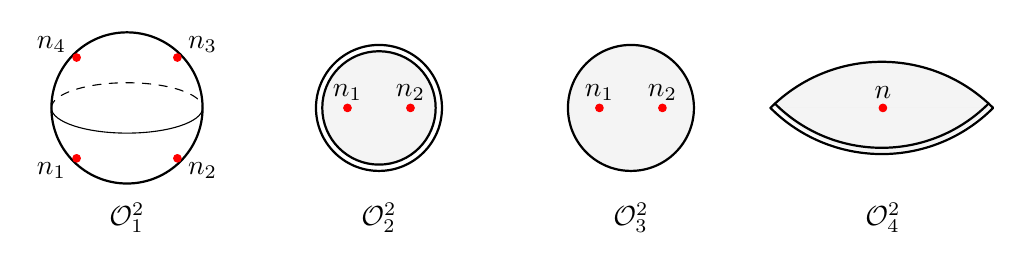
\begin{tikzpicture}[line join = round, line cap = round, scale=.8]
 %
 \begin{scope}[shift={(0,0)}]
 \draw[thick] (0,1) circle(1.2);
     \draw[red, fill=red] (-.8,0.2) circle(0.06);
     \draw[red, fill=red] (.8,0.2) circle(0.06);
     \draw[red, fill=red] (.8,1.8) circle(0.06);
     \draw[red, fill=red] (-.8,1.8) circle(0.06);
      \draw (-1.2,1) arc[x radius = 1.2, y radius = .4, start angle =180, end angle= 360 ];
      \draw[dashed] (-1.2,1) arc[x radius = 1.2, y radius = .4, start angle =180, end angle= 0 ];
     \draw (-6/5,0) node{$n_1 $};
     \draw (6/5,0) node{$n_2 $};
     \draw (6/5,2) node{$n_3 $};
     \draw (-6/5,2) node{$n_4 $};
     \draw (0,-.75) node{$\mathcal O^2_1$};
   \end{scope}
   %
       \begin{scope}[shift={(4,0)}]
        \fill[gray!30!white, opacity=.3] (0,1) circle(.9);
        \draw[thick] (0,1) circle(1);
         \draw[thick] (0,1) circle(.9);
      \draw[red, fill=red] (-.5,1) circle(0.06);
      \draw[red, fill=red] (.5,1) circle(0.06);
    \draw (-.5,1.25) node{$n_1 $};
     \draw (.5,1.25) node{$n_2 $};
     \draw (0,-.75) node{$\mathcal O^2_2$};
   \end{scope}
%
       \begin{scope}[shift={(8,0)}]
        \fill[gray!30!white, opacity=.3] (0,1) circle(1);
        \draw[thick] (0,1) circle(1);
      \draw[red, fill=red] (-.5,1) circle(0.06);
      \draw[red, fill=red] (.5,1) circle(0.06);
    \draw (-.5,1.25) node{$n_1 $};
     \draw (.5,1.25) node{$n_2 $};
     \draw (0,-.75) node{$\mathcal O^2_3$ }; 
   \end{scope}
%
       \begin{scope}[shift={(12,0)}]
\fill[gray!30!white, opacity=.3] (1.75,1)  arc [start angle=45, end angle=135, x radius=2.5cm, y radius =2.5cm] ;
\fill[gray!30!white, opacity=.3]  (1.7,1) arc [start angle=-45, end angle=-135, x radius=2.4cm, y radius =2.4cm] ;
\draw[thick] (1.75,1) arc [start angle=45, end angle=135, x radius=2.5cm, y radius =2.5cm] ;
\draw[thick] (1.75,1) arc [start angle=-45, end angle=-135, x radius=2.5cm, y radius =2.5cm] ;
%
 \draw[thick] (1.678,1.07) arc [start angle=-45, end angle=-135, x radius=2.4cm, y radius =2.4cm] ;
      \draw[red, fill=red] (0,1) circle(0.06);
%       \draw[red, fill=red] (.5,1) circle(0.06);
    \draw (0,1.25) node{$n $};
%      \draw (.5,1.25) node{$n_2 $};
     \draw (0,-.75) node{$\mathcal O^2_4$ }; 
   \end{scope}   
\end{tikzpicture}
\end{center}
\caption{The four examples in Section~\ref{section:Examples}. The orbifold 
$\mathcal O^2_1$ is the orientation covering of 
$\mathcal O^2_2$, and 
$\mathcal O^2_3$, of 
$\mathcal O^2_4$ (for a suitable choice of labels).}
\label{Figure:Exs}
\end{figure}

 
 
 
 
 
 \begin{Example} Consider a sphere with 4 cone points 
  $\mathcal O^2_1=S^2(n_1,n_2,n_3,n_4)$. 
  Since $\mathcal O^2_1$ is hyperbolic, at  
  least one of the $n_i$ is $\geq 2$.
  The dimension of the space of convex projective structures is 
  $\dim  (   \mathrm{Proj}_{\mathrm{cvx}}(\mathcal O^2_1))= 8-2 k $, where 
  $0\leq k\leq 3$ is the number of $n_i$ equal to $2$.
  The dimension of the Teichm\"uller space is 
  $d=\dim (\mathrm{Teich}(\mathcal O^2_1))=2$. 
  
  As $\mathcal O^2_1$ 
  is orientable and closed, $X(\mathcal O^2_1,\mathrm{SL}_4(\mathbb R))$
  has a neighborhood homeomorphic to
 $$ 
\mathbb R^{8-2k}\times  \mathrm{Cone}( \mathrm{UT}( S^{1}))= 
\mathbb R^{8-2k}\times    \mathrm{Cone}( S^{1}  \sqcup S^{1})
   $$
Namely,    the neighborhood is homeomorphic to the union to 2 manifolds of dimension $10-2k$
that intersect transversely along a manifold of codimension 2. 
 \end{Example}

 
 
 
 
 
 
 
 
 
 
 
 
 
 
 
   \begin{Example}
   Consider a disc with mirror boundary and two cone points of 
 order $n_1$ and $n_2$, with at most one of the $n_i$ equal to 2. This is a non-orientable closed 2-orbifold,
 that we denote by  $\mathcal O^2_2=D^2(n_1,n_2;\emptyset)$. Its orientation covering
 is $S^2(n_1, n_1, n_2, n_2)$. Now the dimension of the space of 
 convex projective structures is 
   $\dim  (   \mathrm{Proj}_{\mathrm{cvx}}(\mathcal O^2_2))= 4-2 k $, where 
  $0\leq k\leq 1$ is the number of $n_i$ equal to $2$. The dimension of the 
  Teichm\"uller space is
  $d=\dim (\mathrm{Teich}(\mathcal O^2_2))=1$. 
  
  As $\mathcal O^2_2$ is non-orientable, we distinguish the orientable embedding
  from the type preserving embedding:
  \begin{enumerate}[(i)]
   \item Consider the orientable embedding. A neighborhood in 
   $X(\mathcal O^2_2, \mathrm{SL}_4(\mathbb R))$ is homeomorphic to 
  $$
  \mathbb R^{4-2k}\times  \mathrm{Cone}( S^{0}\times S^0)
  $$
Here  $S^0\times S^0$ is the set with cardinality 4.
Namely,    the neighborhood is homeomorphic to the union to 2 manifolds of dimension $5-2k$ that intersect along a manifold of codimension one.
  \item Consider the type preserving embedding. A neighborhood  of the character  in 
  $X(\mathcal O^2, \mathrm{SL}_{\pm}(4,\mathbb R))$ is homeomorphic to 
  $$
  \mathbb R^{4-2k}\times  \mathrm{Cone}( S^{0}\times S^0)/\!\!\sim\,\, =
    \mathbb R^{4-2k}\times  \mathrm{Cone}(S^{0})\cong  \mathbb R^{5-2k}.
  $$
  Thus the neighborhood is topologically non-singular.
  
  \end{enumerate}
   \end{Example}

  
 

   \begin{Example} Next consider a disc with 
   two cone points of order $n_1$ and $n_2$, with $(n_1,n_2)\neq (2,2)$, 
        $\mathcal O^2_3=D^2(n_1,n_2)$. Even if the underlying space and the number of 
        cone points is the same as the previous one,
        this orbifold is orientable and has boundary. 
        The deformation space however looks like the previous example (orientable embedding):   
        $\dim  (   \mathrm{Proj}_{\mathrm{cvx}}(\mathcal O^2_3))= 4-2 k $, where 
  $0\leq k\leq 1$ is the number of $n_i$ equal to $2$ and 
  $\dim (\mathrm{Teich}(\mathcal O^2_3))=1$.  As $\partial \mathcal O^2_3
  \neq\emptyset$,  $X(\mathcal O^2_3, \mathrm{SL}_4(\mathbb R))$ is again homeomorphic to 
  $
  \mathbb R^{4-2k}\times  \mathrm{Cone}( S^{0}\times S^0)
   $.
   \end{Example}

 
 
   \begin{Example}
   \label{Example:On}
   Consider $\mathcal O^2_4$ a disc $D^2$ with one cone point of order $n\geq 3$
   and $\partial D^2$ is the union of a full orbifold and a mirror interval. 
    This is a non-orientable orbifold with boundary, and its 
    orientation cover is $D^2(n, n)$, the previous example. 
    Now  $\dim  (   \mathrm{Proj}_{\mathrm{cvx}}(\mathcal O^2_4))= 2 $
     and 
     $\dim (\mathrm{Teich}(\mathcal O^2_4))=1$.  
       \begin{enumerate}[(i)]
   \item For the orientable embedding, a neighborhood in
   $X(\mathcal O^2_4, \mathrm{SL}_4(\mathbb R))$ is homeomorphic to 
  $$
  \mathbb R^{2}\times  \mathrm{Cone}( S^{0}\times S^0)
  $$
  and the neighborhood is homeomorphic to the union of two 3-manifolds
  that intersect along a surface.  
  \item Consider the type preserving embedding. As $\mathsf{f}(\partial \mathcal O^2_4)= 1$, 
  $$\dim (\mathrm{Teich}(\mathcal O^2_4))- 
  \mathsf{f}(\partial \mathcal O^2_4)=0.$$
  Thus all deformations of representations of $\pi_1(\mathcal O^2_4)$
  in $\mathrm{SL}^{\pm}_4(\mathbb R)$ remain in
  $\mathrm{SL}^{\pm}_3(\mathbb R)$.
    \end{enumerate}
     
    
     
    
   \end{Example}


\section{Projective deformations of hyperbolic 3-orbifolds}
\label{Section:projdef3}

Consider a hyperbolic 3-orbifold. It has a natural 
projective structure, by using the projective model of hyperbolic geometry,
and there is no known general criterion to determine
the deformation space of those projective structures,
cf.~\cite{CLT1, CLT2, HeusenerPorti11}.
%
% We introduce first the notion of projectively infinitesimally rigidity 
% with respect to the boundary. For finite
% volume manifolds this implies smoothness, see
% \cite{BDL}. Here we consider orbifolds of finite type in general.

\begin{Definition}
A compact hyperbolic 3-orbifold $\mathcal O^3$ is projectively infinitesimally rigid 
with respect to the boundary if 
the inclusion induces an injection
$$
0\to H^1(\mathcal O^3,\mathfrak{sl}(4,
\mathbb R)) \to 
H^1(\partial \mathcal O^3,\mathfrak{sl}(4,
\mathbb R)).
$$
\end{Definition}

For finite volume hyperbolic manifolds, infinitesimally rigid 
with respect to the boundary  was defined  in a joint paper with Heusener 
\cite{HeusenerPorti11}. 
For finite volume hyperbolic manifolds, Ballas,  Danciger,  and Lee 
\cite[Theorem~3.2]{BDL}
proved that infinitesimal rigidity with respect to the boundary implies that the space of 
$\mathrm{PSL}(4,\mathbb R)$ characters is smooth.
Here we consider compact 3-orbifolds with hyperbolic interior, possibly of infinite volume, namely orientable 3-orbifolds of finite type.


\begin{Example}
 Consider a product $\mathcal O^3=\mathcal O^2\times [0,1]$ it is infinitesimally
 projectively rigid for any hyperbolic structure. 
 
When $\mathcal O^2$ is Fuchsian, 
its holonomy is contained in 
$\mathrm{SO}(2,1)\subset\mathrm{SL}_3(\mathbb R)$, hence reducible as representation in 
$\mathrm{SL}_4(\mathbb R)$.  By Theorem~\ref{Theorem:orientable},  the space of characters in 
 $\mathrm{SL}_4(\mathbb R)$ is singular. But when it is quasi-Fuchsian (and non-Fuchsian) it is smooth.
\end{Example}





\begin{Theorem}
\label{Theorem:3dim}
Let $\mathcal O^3$ be a compact orientable orbifold, with $\partial \mathcal O^3\neq \emptyset$, and hyperbolic interior
$\mathrm{int}( \mathcal O^3 )$ so  that it is not elementary, nor Fuchsian.
Assume that $\mathcal O^3$ is infinitesimally projectively rigid 
with respect to the boundary.

Then 
 the character of the
hyperbolic holonomy is a smooth point of
$X(\mathcal O^3, \mathrm{SL}_4(\mathbb R))$
if,  and only if,
all ends of 
$\mathrm{int}( \mathcal O^3 )$ are either non-Fuchsian or turnovers. Furthermore, the singularity is quadratic.
 \end{Theorem}

\begin{Definition}
We say that one end is \emph{Fuchsian} if its holonomy is a Fuchsian group: namely the end corresponding to a totally geodesic 
boundary component.  
\end{Definition}

In this definition, finite volume ends (e.g.~corresponding to
a Euclidean boundary component) are not considered Fuchsian.


\begin{Lemma}
\label{Lemma:03irr}
 Let $\mathcal O^3$ be a compact orientable orbifold, with  hyperbolic interior. If it is not elementary nor 
Fuchsian, then its holonomy
 $\pi_1(\mathcal O^3)\to \mathrm{SO}_0(3,1)\subset
 \mathrm{SL}_4(\mathbb R)$ is $\mathbb C$-irreducible.~
\end{Lemma}


\begin{proof}
 If there is a proper subspace  $V\subset \mathbb C^4$ invariant by the holonomy, then the image of holonomy
 is contained in the  subgroup $G'=\{g\in \mathrm{SO}_0(3,1)\mid g V= V\}$, that has finitely many components. 
 As $\mathbb C^4$ is irreducible as  $\mathrm{SO}_0(3,1)$-module (consider for 
  instance the list of irreducible representations of $\mathrm{(P)SL}(2,\mathbb C)$) the identity component
  $G'_0$  of $G'$ 
 is a proper connected subgroup of $\mathrm{SO}_0(3,1)$. 
  Consider the action of this subgroup $G'_0$ in hyperbolic space: as it is a proper subgroup, $G'_0$  preserves either a totally geodesic plane,
a line,  or a point in either hyperbolic space or the ideal boundary. Then the lemma follows from the discussion of 
the possible extensions of stabilizers of those objects.
\end{proof}





\subsection{Infinitesimal projective rigidity}

% Let us mention an application of Goldman's
% obstructions to deforming projective structures of
% 3-dimensional orbifolds.




% % 
% % Reviewing  \cite{HeusenerPorti11},
% % the Lie algebra decomposes as $\pi_1(\mathcal O^3)$-module as 
% % $\mathfrak{sl}(4, \mathbb R)=\mathfrak{so}(3,1)\oplus V$,
% % where $V$ is the subspace of matrices symmetric for the bilinear form
% % $ \mathrm{diag}(1,1,1,-1)$. The inclusion in cohomology holds true 
% % for $\mathfrak{so}(3,1)$ by infinitesimal rigidity results in hyperbolic geometry and one onluy needs to worry about $V$. The definition
% % stated in  \cite{HeusenerPorti11} is stated 


% 
% \begin{Proposition}
% \label{Theorem:3dim}
% Let $\mathcal O^3$ be a compact orientable orbifold, with $\partial \mathcal O^3\neq \emptyset$, and hyperbolic interior
% $\mathrm{int}( \mathcal O^3 )$.
% Assume that all ends of 
% $\mathrm{int}( \mathcal O^3 )$ are either non-Fuchsian or turnovers. 
% 
% If $\mathcal O^3$ is infinitesimally rigid 
% with respect to the boundary, then the
% hyperbolic holonomy is a smooth point of
% $X(\mathcal O^3, \mathrm{SL}_4(\mathbb R))$.
% \end{Proposition}




Fix the Lie algebra $\mathfrak g= \mathfrak{sl}(4,
\mathbb R)$.
Let $\partial \mathcal O^3= \mathcal O^2_1\cup \cdots \cup  \mathcal O^2_k$ denote the decomposition in 
connected components, so that 
$$
H^*(\partial \mathcal O^3,\mathfrak g)=\bigoplus_{i=1}^k H^*(  \mathcal O^2_i,\mathfrak g) \cong 
\bigoplus_{i=1}^k H^*(\pi_1(   \mathcal O^2_i),\mathfrak g),
$$
where, for each $i$, $\mathfrak g$ is a $\pi_1( \mathcal O^2_i)$-module via the adjoint of
the restriction of $\rho$. The first step of the proof of Theorem~\ref{Theorem:3dim} is the following:


\begin{Lemma}
\label{Lemma:resiso}
Let $\mathcal O^3$ be a compact orientable orbifold, with $\partial \mathcal O^3\neq \emptyset$, and hyperbolic interior
$\mathrm{int}( \mathcal O^3 )$, non-elementary and not a product.
Assume that $\mathcal O^3$ is infinitesimally projectively rigid 
with respect to the boundary. Then:
\begin{enumerate}[(i)]
 \item $\dim H^1(\mathcal O^3,\mathfrak g)=\frac12 \dim H^1(\partial\mathcal O^3,\mathfrak g)$
 \item The restriction induces an isomorphism 
\begin{equation}
\label{eqn:periph}
H^2(\mathcal O^3,\mathfrak g)\cong H^2(\partial\mathcal O^3,\mathfrak g).
 \end{equation}
\end{enumerate}
\end{Lemma} 
 
\begin{proof}[Proof of Lemma~\ref{Lemma:resiso}]
We use the long exact sequence in cohomology of the pair 
$(\mathcal O^3,\partial\mathcal O^3)$ with coefficients in the Lie algebra $\mathfrak g= \mathfrak{sl}(4,
\mathbb R)$. Firstly, by hypothesis, the inclusion induces an injection
$
0\to H^1(\mathcal O^3,\mathfrak{g}) \to 
H^1(\partial \mathcal O^3,\mathfrak{g})
$.
Therefore, by duality the map in the long exact sequence is a surjection:
$
H^1(\partial \mathcal O^3,\mathfrak{g}) \to 
H^2(\mathcal O^3,\partial \mathcal O^3,\mathfrak{g})\to 0
$,
and combining this duality with exactness we get (i).
Again by exactness
$
 H^2(\mathcal O^3,\mathfrak g)\to H^2(\partial\mathcal O^3,\mathfrak g)
$ is an injection.
On the other hand,   $H^3(\mathcal O^3,\mathfrak g)=0$ because $\mathcal O^3$ has 
the homotopy type of a 2-dimensional CW-complex, thus  the isomorphism
$H^2(\mathcal O^3,\mathfrak g)\cong H^2(\partial\mathcal O^3 , 
\mathfrak g)$
follows.
\end{proof}


\begin{proof}[Proof of Theorem~\ref{Theorem:3dim}
when there are no Fuchsian ends]

We prove one implication of the theorem, by using 
Goldman's obstruction theory. Given $z\in Z^1(\pi_1(\mathcal O^3),\mathfrak g)$,
we aim to show that the first obstruction to integrability $[z\cup z]$ and all successive obstructions 
vanish in $  H^2(\pi_1(\mathcal O^3),\mathfrak g)$. Using the isomorphism in \eqref{eqn:periph}
and naturality of the obstructions, it amounts to check that if $z_i$ denotes the restriction
of $z$ to $\pi_1(\mathcal O^2_i)$, then $z_i$ is integrable in 
$\hom(\pi_1(\partial_i\mathcal O^3), 
\mathrm{SL}_4(\mathbb R)
)$ for every $i=1,\ldots ,k$. To prove that 
we distinguish cases according to the geometry of the end of $\mathrm{int}(\mathcal O^3)$ corresponding to
$\mathcal O^2_i$.

First assume that $\mathcal O^2_i$ is Euclidean (eg the corresponding end has finite volume). If $\mathcal O^2$ is a
manifold, then it is a 2-torus and in this case \cite[Lemma~3.4]{BDL} Ballas, Danciger and Lee prove that for a peripheral torus 
the space of representations in $\mathrm{SL}_4(\mathbb R)$ is smooth, 
and the sequence of obstructions to integrability vanishes, see also
\cite[Proof of Theorem~3.2]{BDL}. If the Euclidean  orbifold
$\mathcal O^2_i$ is not a 2-torus, by Bieberbach theorem 
$\mathcal O^2_i$ has a finite regular covering that is a 2-torus $T^2$, and the cohomology of $\mathcal O^2_i$
is equivalent to the equivariant cohomology of $T^2$. So the claim follows  from naturality of the obstruction by a standard 
equivariance argument.


Next assume that $\mathcal O^2_i$ is hyperbolic and the corresponding end is not Fuchsian. Then the holonomy restricted
to $\pi_1(\mathcal O^2_i)$ is $\mathbb C$-irreducible in $\mathrm{SL}_4(\mathbb R)$ and therefore 
$H^2(\pi_1(\mathcal O^2_i),\mathfrak g)=0$. Thus there are no obstructions to integrability of $z_i$  at all. 

When $\mathcal O^2_i$ is a turnover, again the space of representations in $\mathrm{SL}_4(\mathbb R)$ is smooth, 
by Corollary~\ref{Corollary:turnover}. So there are no obstructions to integrability

Once the obstructions to integrability in 
$H^2(\mathcal O^3,\mathfrak g)$ vanish, it is a standard argument to prove smoothness, see \cite{Goldman,HPS} 
for instance.
 \end{proof}
% 
% 
% 
% ***************************************************************************
% 
% 


\subsection{Hyperbolic 3-orbifolds with Fuchsian ends}




\begin{proof}[Proof of Theorem~\ref{Theorem:3dim}
 when there are Fuchsian ends]

Firstly  we prove that there is a singularity, by deforming the hyperbolic structure to another hyperbolic structure with
no Fuchsian ends and comparing the dimension of the Zariski tangent space.


\begin{Lemma}
\label{Lemma:NFD}
There is a deformation of the hyperbolic structure of $\mathcal O^3$ (eg a deformation in $\hom(\pi_1(\mathcal O^3),\mathrm{SO}(3,1))$)
 such that none of the ends is Fuchsian.
 \end{Lemma}

\begin{proof}
Here we use 
the complex structure of the group of orientation preserving
isometries of hyperbolic space, as the identity component of $\mathrm{SO}(3,1)$ is isomorphic to $\mathrm{PSL}(2,\mathbb C)$.
In a neighborhood of the hyperbolic holonomy,
the variety of characters
$X(\mathcal O^3,\mathrm{PSL}(2,\mathbb C))$
is a smooth complex variety of positive dimension
\cite[Section~8.8]{KapovichBook}. Thus there are non-trivial deformations.
If a path of deformations stays Fuchsian in one end,
then its restriction to this end is conjugate to a
representation in  $\mathrm{PSL}(2,\mathbb R)$.
If one multiplies the tangent vector to this deformation 
by a complex number with non-zero imaginary part, then one obtains an infinitesimal deformation to a non-Fuchsian representation. 
As there are finitely many ends, there exists a direction
that is non-Fuchsian for every end.
\end{proof}



Now we aim to show that along the deformation of the previous lemma the dimension of the Zariski tangent space decreases strictly. The steps of the proof are the following:
\begin{enumerate}[(1)]
 \item Infinitesimal projective rigidity is an open condition
 in the variety of representations $\hom(\pi_1(\mathcal O^3),\mathrm{SO}(3,1))$. This follows from semi-continuity. 
 \item  By Lemma~\ref{Lemma:resiso}, $\dim H^1(\mathcal O^3,\mathfrak g)=\frac12 \dim H^1(\partial\mathcal O^3,\mathfrak g)$
 for any infinitesimal projectively rigid representation in 
 $\mathrm{SO}(3,1)$.
 
 \item  Let $\rho_0\colon \pi_1(\mathcal O^2_i)\to\mathrm{SO}(2,1)$ be a Fuchsian representation and consider $\rho'\colon \pi_1(\mathcal O^2_i)\to\mathrm{SO}(3,1)$ a non-Fuchsian deformation of  $\rho_0$. Then
 $$
 \dim H^1(\mathcal O^2_i, \mathfrak{sl}_4(\mathbb R)_{\mathrm{Ad}\rho'})
 =
  \dim H^1(\mathcal O^2_i, \mathfrak{sl}_4(\mathbb R)_{\mathrm{Ad}\rho_0})-2
 $$
\end{enumerate}
These   items  imply that
the dimension of the Zariski tangent space decreases under the deformation
of Lemma~\ref{Lemma:NFD}, hence it is singular.  To prove Item~(3), notice that
the quantity
$$
\sum_j \dim (-1)^j \dim H^j(\mathcal O^2_i, \mathfrak{sl}_4(\mathbb R)_{\mathrm{Ad}\rho})
$$
is constant under deformations of $\rho$, 
by \eqref{eqn:twistedEuler}. Thus Item~(3) follows from Poincar\'e duality and
$$
 H^0(\mathcal O^2_i, \mathfrak{sl}_4(\mathbb R)_{\mathrm{Ad}\rho})\cong
  \mathfrak{sl}_4(\mathbb R)^{\mathrm{Ad}\rho}
 \cong
 \begin{cases}
  \mathbf{m}_0\cong \mathbb R & \textrm{ if } \rho \textrm{ is Fuchsian,}\\
  0 & \textrm{ otherwise.}
 \end{cases}
$$

% \begin{Lemma}
% 
% \end{Lemma}
% 
% 
% 
% Then the argument follows from the previous case 
% as the dimension is less than the dimenison of the Zariski tangent space.

\bigskip



Next we show that the singularity is quadratic.
To avoid technicalities, we work with the complexification,
namely the variety or representations in 
$\mathrm{SL}_4(\mathbb C)$ instead of 
$\mathrm{SL}_4(\mathbb R)$. This is sufficient
to get quadratic singularities, by \cite[\S 3.3]{GoldmanMillson}. 

By Lemma~\ref{Lemma:03irr} the holonomy of 
$\mathcal O^3$ is $\mathbb C$-irreducible,
and by Theorem~\ref{Theorem:slices}
there exists an analytic slice $\mathcal S$ at $\rho$ that satisfies:
% as in Theorem~\ref{Theorem:slices}.
$$T_\rho^{\mathrm{Zar}} \mathcal S\oplus B^1(\pi_1(\mathcal O^3),
\mathfrak{sl}_4(\mathbb C))=
Z^1(\pi_1(\mathcal O^3),
\mathfrak{sl}_4(\mathbb C)),
$$
hence $ 
T_\rho^{\mathrm{Zar}} \mathcal S\cong H^1(\pi_1(\mathcal O^3),
\mathfrak{sl}_4(\mathbb C))
$.
By \cite[Theorem~V.A.14]{GunningRossi}
a $\mathcal S$ is equivalent to a subvariety of a (non-singular) 
$\mathbb C$-manifold that has the same dimension  as the Zariski tangent space
of the analytic germ. So 
there exist germs of non-singular
$\mathbb C$-subvarieties  $M$, $M_1,\ldots,M_k$, such that, after taking
a  small enough slice and choosing neighborhoods $\rho\vert_{\pi_1 O^2_i}
\in U_i\subset  \hom(\pi_1(\mathcal O^2_i),\mathrm{SL}_4(\mathbb C))$ we have:
\begin{align*}
\rho\in \mathcal S\subset M,  & \qquad T_\rho^{\mathrm{Zar}} \mathcal S=T_\rho M,  \\
 \rho_i\in U_i\subset M_i, & \qquad T_{\rho\vert _{\pi_1\mathcal O^2_i} } \hom(\pi_1(\mathcal O^2_i),\mathrm{SL}_4(\mathbb C)) =T_{\rho\vert _{\pi_1\mathcal O^2_i}} M_i.
\end{align*}
% $$
% S\subset M\quad\textrm{ and }\quad 
% T_\rho S=T_\rho M\qquad 
% $$
% and 
% $$
% U_i\subset M_i
% \quad\textrm{ and }\quad 
% T_{\rho\vert _{\pi_1\mathcal O^2_i} } \hom(\pi_1(\mathcal O^2_i),\mathrm{SL}_4(\mathbb C)) =T_{\rho\vert _{\pi_1\mathcal O^2_i}} M_i.
% $$
% 
% 
% $$ (by taking $S$ smaller if necessary), a neighborhood
% $\rho\vert_{\pi_1 O^2_i}
% \in U_i\subset  \hom(\pi_1(\mathcal O^2_i),\mathrm{SL}_4(\mathbb C))$ so that $U_i\subset M_i$ and 
% % $$
% % T_\rho S=T_\rho M\qquad \textrm{ and }\qquad  T_{\rho\vert _{\pi_1\mathcal O^2_i} } \hom(\pi_1(\mathcal O^2_i),\mathrm{SL}_4(\mathbb C)) =T_{\rho\vert _{\pi_1\mathcal O^2_i}} M_i.
% % $$
The restriction map
$$
\mathcal 
S\to \prod_i U_i\subset\prod_i \hom(\pi_1(\mathcal O^2_i),\mathrm{SL}_4(\mathbb C))
$$
is analytic, hence it extends to % \cite[Theorem~V.A.14]{GunningRossi} to 
$$
\phi\colon M\to \prod_i M_i
$$
and since the restriction induces an injection 
$$
H^1(\mathcal O^3,\mathfrak{sl}_4(\mathbb C))
\to
\bigoplus_i 
H^1(\mathcal O^2_i,\mathfrak{sl}_4(\mathbb C) )
$$
the map $\phi \colon M\to \prod_i M_i$ is an analytic injection. The  following lemma implies that the singularity of $\mathcal S$ at $\rho$ is quadratic,
as each  $\hom(\pi_1(\mathcal O^2_i),\mathrm{SL}_4(\mathbb C))$ (or $U_i$)
is quadratic in $M_i$:

\begin{Lemma}
  $\phi(\mathcal S)=\phi(M)\cap \prod_i \hom(\pi_1(\mathcal O^2_i),\mathrm{SL}_4(\mathbb C))$.
\end{Lemma}





% % 
% % is an analytic submanifold $S\subset M\subset \hom(\pi_1(\mathcal O^3),\mathrm{SL}_4(\mathbb C))$ (eg non-singular) such that
% % $T_\rho S=T_\rho M$. 
% % 
% % Again by \cite[Theorem~V.A.14]{GunningRossi}
% % there is a smooth manifold $M_i$ such that
% % $ \hom(\pi_1(\mathcal O^2_i).\mathrm{SL}_4(\mathbb R))\subset M_i$, and
% %  
% % 
% % GR:
% % $S\subset M$ analytic manifold, $TS=TM$
% % $ \hom(\pi_1(\mathcal O^2_i).\mathrm{SL}_4(\mathbb R))\subset M_i$
% 
% $S\to \prod_i \hom(\pi_1(\mathcal O^2_i).\mathrm{SL}_4(\mathbb R))$
% extends to 
% $M\to \prod_i M_i$ by analycity. It is an
% immersion (by inf proj rigidity)
% 
% \begin{Lemma}
%  $S=M\cap \prod_i \hom(\pi_1(\mathcal O^2_i).\mathrm{SL}_4(\mathbb R))$
% \end{Lemma}


\begin{proof}[Proof of the lemma]
By construction we have the inclusion
 $$\phi(\mathcal S)\subseteq\phi(M)\cap \prod_i \hom(\pi_1(\mathcal O^2_i),\mathrm{SL}_4(\mathbb C))$$
and we prove equality
by contradiction. Assume
$$\phi(\mathcal S)\subsetneq\phi(M)\cap \prod_i \hom(\pi_1(\mathcal O^2_i),\mathrm{SL}_4(\mathbb C)).$$ 
Then there exists a $(k+1)$-jet 
$$
c=c_0+c_1 t+\cdots + c_{k+1} t^{k+1}
\in J^{k+1}_{0,\phi(\rho)}\big(\mathbb R,   \phi(M)\cap \prod_i \hom(\pi_1(\mathcal O^2_i),\mathrm{SL}_4(\mathbb C) )\big)  
$$ 
such that
$c$ is not a $(k+1)$-jet of $\phi(\mathcal{S})$,
$c \not\in 
 J^{k+1}_{0,\phi(\rho)}(\mathbb R,   \phi(\mathcal{S}))$,
but 
its $k$-th truncation is:
$$
[c]_k=c_0+c_1 t+\cdots + c_{k} t^{k}
\in J^{k}_{0,\phi(\rho)}(\mathbb R,   \phi(\mathcal{S})).
$$
We write $[c]_k=\phi( \rho_k)$ for some $k$-jet in the slice $\rho_k\in J^k_{0, \rho}(\mathbb R, \mathcal S)$, that in its turn we write as
$$
\rho_k=\exp(a_1 t+\cdots a_k t^k)\rho \in J^{k+1}_{0,\rho} (\mathbb R, \mathcal S)
$$
for some maps (or 1-cochains) $a_i\colon\Gamma \to \mathfrak{sl}_4(\mathbb C)$.
By Goldman's theory \cite{Goldman,HPS},
the obstruction to extend $\rho_k$ to a $(k+1)$-jet
is a cohomology class in $H^2(\mathcal O^3,\mathfrak{sl}_4(\mathbb C))$.
By  Lemma~\ref{Lemma:resiso} the restriction map induces an isomorphism 
$H^2(\mathcal O^3,\mathfrak{sl}_4(\mathbb C))\cong H^2(\partial\mathcal O^3,\mathfrak{sl}_4(\mathbb C))$.
Thus, by naturality of the obstruction and since $[c]_k$ is the truncation of the $(k+1)$-jet $c$, this obstruction vanishes
in $H^2(\mathcal{O}^3,\mathfrak{sl}(4,\mathbb C))$. 
Therefore $\rho_k$ is the $k$-truncation of a $(k+1)$-jet:
$$
\rho_{k+1}=\exp(a_1 t+\cdots a_k t^k+a_{k+1} t^{k+1} ) \rho \in J^{k+1}_{0,\rho} 
\big(\mathbb R, \hom(\pi_1 \mathcal O^3, \mathrm{SL}_4(\mathbb C) )\big) 
$$
Next we want to conjugate $\rho_{k+1}$ so that the result is not only a jet in
$ \hom(\pi_1 \mathcal O^3, \mathrm{SL}_4(\mathbb C) )$ but in
the slice $\mathcal S$. For than purpose we use
Theorem~\ref{Theorem:slices}~(ii): 
a neighborhood of $\rho$ in $ \hom(\pi_1 \mathcal O^3, \mathrm{SL}_4(\mathbb C) )$
is obtained by conjugating 
the slice $\mathcal S$ by a neighborhood of the origin in $\mathrm{SL}_4(\mathbb C) $. Thus we write
$$
\rho_{k+1}=\operatorname{Ad}_{\exp (t^{k+1} b)} \rho_{k+1}'
$$
with $b\in\mathfrak{sl}_4(\mathbb C)$ and $\rho_{k+1}'   $  a jet in the slice $\mathcal S$
(whose $k$ truncation is $\rho_k$):
$$
\rho_{k+1}'=
\exp(a_1 t+\cdots a_k t^k+a_{k+1}' t^{k+1} ) \rho \in J^{k+1}_{0,\rho} (\mathcal{S}) .
$$
% By construction, the difference $a_{k+1}-a_{k+1}'$ is the inner cocycle corresponding 
% to
% $b\in\mathfrak{sl}_4(\mathbb C)$, thus
% we consider 
% $$\rho_{k+1}'=  \operatorname{Ad}_{\exp (-t^{k+1} b)}
% \rho_{k+1}.
% $$
% 
% after conjugating by $\exp (-t^{k+1} b)$
% we may assume that $\rho_{k+1}$ is already a jet in the slice:  
% $$
% \rho_{k+1}\in J^{k+1}_{0,\rho} (\mathcal{S}). 
% $$
Notice that $\phi(\rho_{k+1}')$ and $c$ are two $(k+1)$-jets
in $\phi(M)$
whose $k$-truncations
are the same, hence their difference is $t^{k+1} v$ for some $v\in T_ {\phi(\rho)}\phi(M)$, namely 
$v=\phi_*(u)$ for some $u\in T_\rho M$. As $T_\rho M=T_\rho S$, we use $u$ it to modify the 
$(k+1)$-the term of $\rho_{k+1}'$ and define:
$$
\rho_{k+1}''=\exp(t^{k+1} u)\rho_{k+1}'=\exp(a_1 t+\cdots a_k t^k+(a_{k+1}'+u) t^{k+1})\rho \in J^{k+1}_{0,\rho} (\mathcal{S}) .
$$
This $(k+1)$-jet satisfies $\phi( \rho_{k+1}'')= c$, hence a contradiction.
% % % 
% % % % but $c(t) \not\in 
% % % %  J^{k+1}_{0,\phi(\rho)}(\mathbb R,   \phi(\mathcal{S}))$
% % % 
% % % To prove equality, we use Goldman obstruction theory. 
% % % By  Lemma~\ref{Lemma:resiso} the restriction map induces an isomorphism 
% % % $H^2(\mathcal O^3,\mathfrak g)\cong H^2(\partial\mathcal O^3,\mathfrak g)$.
% % % Hence,  each germ of analytic path in 
% % % $\phi(M)\cap \prod_i \hom(\pi_1(\mathcal O^2_i),\mathrm{SL}_4(\mathbb C))$ is in fact a germ of analytic path in $\phi(\mathcal{S})$, thus the equality.
\end{proof}




By the properties of the slice in Theorem~\ref{Theorem:slices}, the singularity at the varieties of characters is quadratic. 
\end{proof}

% % 
% % \begin{Theorem}
% % \label{Theorem:QuasifuchsianSingular}
% % Let $\mathcal O^3$ be an orientable hyperbolic orbifold of infinite volume, with at least one end that is Fuchsian and different from a turnover.
% % Then its hyperbolic  holonomy has a non-integrable  infinitesimal deformation in $\mathrm{SL}_4(\mathbb R)$. 
% % % % \begin{enumerate}[(i)]
% % % %  \item Its hyperbolic  holonomy has a non-integrable  infinitesimal deformation in $\mathrm{SL}_4(\mathbb R)$. 
% % % % \item If in addition $\mathcal O^3$ is infinitesimally rigid 
% % % % with respect to the boundary, then the character of the hyperbolic holonomy is
% % % % singular in $X(\mathcal O^3, \mathrm{SL} (4,\mathbb R))$
% % % % \end{enumerate}
% % \end{Theorem}
% % Before proving the theorem  we consider some further decompositions of Lie algebras. Set 
% %  $$J= \mathrm{diag}(-1,1,\ldots,1),$$ 
% %  so that 
% %  $$\mathfrak{so}(n,1)=\{ a\in \mathfrak{sl}(n+1,\mathbb R) 
% %  \mid a^t = - J a J\}.
% %  $$
% %  We are mainly interested inthe cases $n=2,3$.
% % Let  
% % $$\mathbf{sym}(n,1)= \{ a\in \mathfrak{sl}(n+1,\mathbb R) 
% %  \mid a^t =  J a J\}$$
% % denote the subspace of $J$-symmetric matrices, hence
% % $$
% % \mathfrak{sl}(n+1,\mathbb R)= \mathfrak{so}(n,1) \perp \mathbf{sym}(n,1)
% % $$
% % is a direct sum  of $\mathrm{SO}(n,1)$-modules  orthogonal by the Killing form. 
% % 
% % Next consider  
% % $$
% % \mathbf m_{\mathfrak{so}}= (  \mathbf m_{\mathsf c}\oplus\mathbf m_{\mathsf r} )\cap \mathfrak{so}(3,1)\quad\textrm{ and }\quad \mathbf m_{ \mathsf{sym}}= (  \mathbf m_{\mathsf c}\oplus\mathbf m _{\mathsf r} )\cap \mathbf{sym}(3,1)
% % $$ 
% % so
% % that 
% % $$
% % \mathbf m_{\mathsf c}\oplus\mathbf m _{\mathsf r}= 
% % \mathbf m_{\mathfrak{so} } \perp \mathbf m_{ \mathsf{sym}}
% % $$
% % as $\mathrm {SO}(2,1)$-modules. Combining these direct sums and 
% % \eqref{eqn:directsum},
% % we have the decompositions of 
% % $\mathrm {SO}(2,1)$ -modules:
% % \begin{align}
% %  \label{eqn:so}
% %  \mathfrak{so}(3,1)&=\mathfrak{so}(2,1)\perp \mathbf m_{\mathfrak{so}}
% % % \qquad\textrm{ and }
% % \\
% %  \label{eqn:sym}
% % \mathbf{sym}(3,1)&= \mathbf{sym}(2,1)\perp \mathbf m_{ \mathsf{sym}} \perp 
% % \mathbf d.
% % \end{align}
% % We have isomorphisms of 
% % $\mathrm {SO}(2,1)$ -modules:
% % $$
% % \mathbf m_{\mathsf c}\cong \mathbf m _{\mathsf r}\cong 
% % \mathbf m_{\mathfrak{so} } \cong  \mathbf m_{ \mathsf{sym}}
% % \cong \mathfrak{so}(2,1).
% % $$
% % The isomorphism 
% % $\mathbf m_{\mathsf c}\cong \mathbf m _{\mathsf r}$ as 
% % $\mathrm {SO}(2,1)$-modules follows from the fact that the contregradient action on $\mathrm {SO}(2,1)$ (transpose and inverse)
% % consists in conjugation by $J$. 
% % 
% % 
% % 
% % 
% % \begin{proof}[Proof of Theorem~\ref{Theorem:QuasifuchsianSingular} (i)]
% % We consider the connected sum decomposition of $\partial\mathcal O^3$,
% % $$
% % \partial \mathcal O^3= \mathcal O^2_1\sqcup\cdots\sqcup
% % \mathcal O^2_k\sqcup \mathcal F^2_1\sqcup\cdots\sqcup \mathcal F^2_l,
% % $$
% % where the  $\mathcal F^2_i$ denote the boundary components different from a turnover corresponding to a Fuchsian end (with $k\geq 0$ and $l \geq 1$).
% % 
% % % % Consider the map 
% % % % $\mathrm{res}\colon H^1(\mathcal O^3,\mathfrak{so}(3,1))\to 
% % % % \oplus_i   H^1(\mathcal F^2_i,\mathfrak{so}(3,1))$ induced by restriction, and 
% % % % the projection 
% % % % $\oplus_{i=1}^l   H^1(\mathcal F^2_i,\mathfrak{so}(3,1))\to
% % % % \oplus_{i=1}^l   H^1(\mathcal F^2_i,\mathbf m_{\mathfrak{so}})
% % % $ form the diect sum ***.
% % 
% % \begin{Lemma}
% % \label{Lemma:res}
% % Let $\mathrm{res}_{\mathcal F}$ denote the map in cohomology induced by restriction and
% % $\pi_{\mathbf m_{\mathfrak{so}}} $ the projection 
% %  induced by \eqref{eqn:so} and 
% % $\pi_{\mathbf m_{\mathsf{sym}}} $ 
% %  the projections induced by \eqref{eqn:sym}.
% % \begin{enumerate}[(i)]
% %               \item 
% %               The composition 
% % $$
% % \pi_{\mathbf m_{\mathfrak{so}}}
% % \circ\mathrm{res}_{\mathcal F}\colon H^1(\mathcal O^3,\mathfrak{so}(3,1))\to 
% % \bigoplus_{i=1}^l   H^1(\mathcal F^2_i,\mathfrak{so}(3,1))
% % \to 
% % \bigoplus_{i=1}^l   H^1(\mathcal F^2_i,\mathbf m_{\mathfrak{so}})
% % $$
% % %            Consider the map 
% % % $\mathrm{res}\colon H^1(\mathcal O^3,\mathfrak{so}(3,1))\to 
% % % \oplus_i   H^1(\mathcal F^2_i,\mathfrak{so}(3,1))$ induced by restriction, and 
% % % the projection 
% % % $\oplus_{i=1}^l   H^1(\mathcal F^2_i,\mathfrak{so}(3,1))\to
% % % \oplus_{i=1}^l   H^1(\mathcal F^2_i,\mathbf m_{\mathfrak{so}})
% % % $ from the direct sum ***.
% % %  The composition 
% % %  $$\pi\circ\mathrm{res}\colon H^1(\mathcal O^3,\mathfrak{so}(3,1))\to 
% % % \oplus_{i=1}^l   H^1(\mathcal F^2_i,\mathbf m_{\mathfrak{so}})
% % % $$ 
% % is surjective. 
% % 
% %  \item 
% % %           Let 
% % % $\mathrm{res}\colon H^1(\mathcal O^3,\mathbf{sym}(3,1))\to 
% % % \oplus_i   H^1(\mathcal F^2_i,\mathbf{sym}(3,1)$ denote now the map induced by restriction, and 
% % % $\oplus_{i=1}^l   H^1(\mathcal F^2_i,\mathbf{sym}(3,1))\to
% % % \oplus_{i=1}^l   H^1(\mathcal F^2_i,\mathbf m_{ \mathsf{sym}})
% % % $, the projection (induced by the direct sum.
% %  The composition 
% % $$
% % \pi_{\mathbf m_{\mathsf{sym}}}
% % \circ\mathrm{res}_{\mathcal F}\colon H^1(\mathcal O^3, \mathbf{sym}(3,1) )\to 
% % \bigoplus_{i=1}^l   H^1(\mathcal F^2_i, 
% % \mathbf{sym}(3,1)  ) 
% % \to 
% % \bigoplus_{i=1}^l   H^1(\mathcal F^2_i,  \mathbf m_{ \mathsf{sym}})  
% % $$ has rank 
% % $\mathrm{ rank}(\pi_{\mathbf m_{\mathsf{sym}}}
% % \circ\mathrm{res}_{\mathcal F})\geq \frac 12 \sum_i
% % \dim  H^1(\mathcal F^2_i,  \mathbf m_{ \mathsf{sym}})$.
% % 
% % \end{enumerate}
% % \end{Lemma}
% % 
% % 
% % We assume the lemma and prove Theorem~\ref{Theorem:QuasifuchsianSingular}. 
% % Let 
% % $$
% % b\colon H^1(\mathcal O^3,\mathfrak{sl}(4))\times H^1(\mathcal O^3,\mathfrak{sl}(4)   )\to H^2(\mathcal O^3,\mathfrak{sl}(4)   )
% % $$
% % denote the bilinear form defined by $b(\theta_1,\theta_2)=[\theta_1\cup\theta_2]$, 
% % i.e. $b(\theta,\theta)$ is the first obstruction to integrability of $\theta$. 
% % By naturality
% % $$
% % \mathrm{res}_{\partial \mathcal O^3}\circ b=
% % \sum_i b \circ\mathrm{res}_{\mathcal O_i^2}+\sum_j  b \circ\mathrm{res}_{\mathcal F_j^2}
% % $$
% % where $b$ denotes the bilinear form in the cohomology of the corresponding orbifold. 
% % Each bilinear form $ b \circ\mathrm{res}_{\mathcal O_i^2}$
% % vanishes, by the discussion in the proof of Proposition~\ref{Theorem:3dim}.
% % Furthermore, 
% %  $$ b \circ\mathrm{res}_{\mathcal F_j^2}= b'_j \circ\pi\circ\mathrm{res}_{\mathcal F_j^2}
% %  $$ 
% % where 
% % $$
% % \pi_{  \mathbf m_{\mathsf r}\oplus \mathbf m_{\mathsf c} } \colon H^1(\mathcal F^2_j,\mathfrak{sl}(4))\to H^1(\mathcal F^2_j,\mathbf m_{\mathsf r}\oplus
% % \mathbf m_{\mathsf c}
% % )
% % $$ 
% % is the projection induced by \eqref{eqn:directsum}
% % and 
% % $$
% % b'_j\colon H^1(\mathcal F^2_j,\mathbf m_{\mathsf r}\oplus \mathbf m_{\mathsf c})
% % \times H^1(\mathcal F^2_j,\mathbf m_{\mathsf r}\oplus \mathbf m_{\mathsf c})
% % \to H^2(\mathcal F^2_j,\mathbf d)\cong \mathbb R
% % $$
% % is a perfect pairing, by Lemma~\ref{Lemma:cupprodcut}.
% % So consider the direct sum of bilinear forms 
% % $$
% % b'=b'_1\oplus\cdots\oplus b'_l\colon 
% % \bigoplus_{i=1}^l   H^1(\mathcal F^2_i,\mathbf m_{\mathsf r}\oplus \mathbf m_{\mathsf c})
% % \times
% % \bigoplus_{i=1}^l   H^1(\mathcal F^2_i,\mathbf m_{\mathsf r}\oplus \mathbf m_{\mathsf c})
% % \to\mathbb R
% % $$
% % By construction $ b'$ is a perfect pairing, and 
% % $$
% % \mathrm{res}_{\mathcal \partial O^3}\circ b=
% % b'\circ 
% % \bigoplus_{j=1}^l (\pi \circ\mathrm{res}_{\mathcal F_j} )
% % $$
% % % where   the map
% % % $$
% % % \pi\circ\mathrm{res}_{\mathcal F}\colon H^1(\mathcal O^3,\mathfrak{sl}(4))\to 
% % % \bigoplus_{i=1}^l   H^1(\mathcal F^2_i,\mathfrak{sl}(4))
% % % \to 
% % % \bigoplus_{i=1}^l   H^1(\mathcal F^2_i,\mathbf m_{\mathsf r}\oplus
% % % \mathbf m_{\mathsf c}
% % % ).
% % % $$
% % By Lemma~\ref{Lemma:res}
% % \begin{multline*}
% % \mathrm{rank}\big (  \bigoplus_{j=1}^k (\pi_{  \mathbf m_{\mathsf r}\oplus \mathbf m_{\mathsf c} } \circ\mathrm{res}_{\mathcal F_j} ) \big) 
% % =
% % \mathrm{rank}\big (
% % \pi_{\mathbf m_{\mathfrak{so}}}
% % \circ\mathrm{res}_{\mathcal F} \big)
% % +
% % \mathrm{rank}\big (
% % \pi_{\mathbf m_{\mathsf{sym}}}
% % \circ\mathrm{res}_{\mathcal F} \big)
% % \\
% %  \geq \sum_i\dim  H^1(\mathcal F^2_i,  \mathbf m_{\mathfrak{so}})+
% % \frac12 \sum_i\dim  H^1(\mathcal F^2_i,  \mathbf m_{\mathsf{sym}})
% % %  \\
% % =
% % \frac34 \sum_i\dim  H^1(\mathcal F^2_i,   \mathbf m_{\mathsf r}\oplus
% % \mathbf m_{\mathsf c}   ) 
% % \end{multline*}
% % %
% % Thus the image of $ \bigoplus_{j=1}^k (\pi_{  \mathbf m_{\mathsf r}\oplus \mathbf m_{\mathsf c} } \circ\mathrm{res}_{\mathcal F_j} )$
% % cannot be isotropic for the perfect pairing $b'$, because its rank is larger than half the dimension of the space. So there exist an element $\theta$ in the image 
% % of $ \bigoplus_{j=1}^k (\pi \circ\mathrm{res}_{\mathcal F_j} ) \big) $ so that
% % $b'(\theta,\theta)\neq 0$, and the theorem is proved.
% % % 
% % % ************
% % % 
% % % 
% % % 
% % % By Lemma~\ref{Lemma:res}, and using the decomposition of
% % % $\mathfrak{sl}(4)$ as $\mathrm{SO}(2,1)$-module,  the map
% % % $$
% % % \pi\circ\mathrm{res}_{\mathcal F}\colon H^1(\mathcal O^3,\mathfrak{sl}(4))\to 
% % % \bigoplus_{i=1}^l   H^1(\mathcal F^2_i,\mathfrak{sl}(4))
% % % \to 
% % % \bigoplus_{i=1}^l   H^1(\mathcal F^2_i,\mathbf m_{\mathsf r}\oplus
% % % \mathbf m_{\mathsf c}
% % % )
% % % $$
% % % has rank $\geq \frac32 \sum_i\dim  H^1(\mathcal F^2_i,  \mathbf m)=
% % % \frac34 \sum_i\dim  H^1(\mathcal F^2_i,   \mathbf m_{\mathsf r}\oplus
% % % \mathbf m_{\mathsf c}   )$.
% % % 
% % % 
% % % Consider $i^*\colon H^1(\mathcal O^3,\mathfrak{sl}(4))
% % % \to  H^1(\partial\mathcal O^3,\mathfrak{sl}(4)   )$ the map induced by inculsion. We want to show that the first obstruction to integrability does not vanish on the image of $i^*$. By naturality, this claim willl imply that the obstruction does not vanish on  $H^1(\mathcal O^3,\mathfrak{sl}(4))$.
% % % This obstruction is the sum of obstructions on each component 
% % %  $\mathcal O^2_ i$ and $\mathcal F^2_ i$.
% % % It vanishes on each $\mathcal O^2_i $ 
% % % (see the discussion in the proof of Proposition~\ref{Theorem:3dim}).
% % % Furthermore, by Lemma~\ref{Lemma:cupprodcut} the obstruction can be computed by projecting to
% % % $\bigoplus_{i=1}^l   H^1(\mathcal F^2_i,\mathbf m_{\mathsf r}\oplus
% % % \mathbf m_{\mathsf c}
% % % )$, and the obstruction to that espace 
% % %  is equivalent to a non-degenerate skew-symmetric pairing.
% % % Now, the map $\pi\circ\mathrm{res}$ has rank
% % % at least $3/4$ the dimension of the space, thus 
% % % the image of  $\pi\circ\mathrm{res}$ cannot be isotropic.  
% % \end{proof}
% % 
% % 
% % 
% % \begin{proof}[Proof of Lemma~\ref{Lemma:res}]
% % (i) We first claim the equality
% % \begin{equation}
% %  \label{egn:infgeod}
% % \dim\ker(\pi_{\mathbf m_{\mathfrak{so}}}\circ \mathrm{res})= \frac 12
% % \sum_{i=1}^k\dim H^1(\mathcal O^2_i,\mathfrak{so}(3,1)),
% %  \end{equation}
% % which vanishes if $k=0$ or all  $\mathcal O^2_i$ are turnovers. 
% % An infinitesimal deformation in 
% % $\ker(\pi\circ \mathrm{res})$ is an infinitesimal hyperbolic deformation that keeps the components $\mathcal F^2_i$ Fuchsian. 
% % Let   $D\mathcal O^3$ denote the double of $\mathcal O^3$ along the Fuchsian components 
% % and $\sigma\colon D\mathcal O^3\to D\mathcal O^3$ the involution that switches components
% % (hence it is locally a reflection along the totally geodesic $\mathcal F^2_i $). So this kernel is isomorphic to the $\sigma$-invariant infinitesimal deformation space of
% % $D\mathcal O^3$:
% % $$
% % \ker(\pi_{\mathbf m_{\mathfrak{so}}}\circ \mathrm{res})\cong H^1(D\mathcal O^3,\mathfrak{so}(3,1))^\sigma
% % $$
% % Now we use the complex structure of the group of orientation preserving
% % isometries of hyperbolic space, as the identity component of $\mathrm{SO}(3,1)$ is isomorphic to $\mathrm{PSL}(2,\mathbb C)$. The tangent space to 
% % $X(D\mathcal O^3, \mathrm{SO}(3,1))\cong X( D\mathcal O^3,
% % \mathrm{PSL}(2,\mathbb C) )$ is 
% % $H^1(D\mathcal O^3,\mathfrak{sl}(2,\mathbb C))$ and 
% % $$
% % \dim_{\mathbb C} H^1(D\mathcal O^3,\mathfrak{sl}(2,\mathbb C))=
% % \frac12\dim_{\mathbb C} H^1(\partial (D\mathcal O^3),\mathfrak{sl}(2,\mathbb C))
% % =
% % \sum_i \dim_{\mathbb C} H^1(\mathcal O^2_i ,  \mathfrak{sl}(2,\mathbb C))
% % $$
% % The involution $\sigma$ acts anti-holomorphically on 
% % $X( D\mathcal O^3,
% % \mathrm{PSL}(2,\mathbb C) )$, because it reverses the orientation, therefore:
% % \begin{multline*}
% % \dim_{\mathbb R}    H^1(D\mathcal O^3,\mathfrak{sl}(2,\mathbb C))^\sigma
% % =
% % \dim_{\mathbb C} H^1(D\mathcal O^3,\mathfrak{sl}(2,\mathbb C))
% % \\ =
% % \sum_i \dim_{\mathbb C} H^1(\mathcal O^2_i ,  \mathfrak{sl}(2,\mathbb C))
% % =
% % \frac12
% % \sum_i \dim_{\mathbb R} H^1(\mathcal O^2_i ,  \mathfrak{so}(3,1)),
% % \end{multline*}
% % which proves \eqref{egn:infgeod}. 
% % 
% % Using that  $
% % \dim H^1(\mathcal O^3 ,  \mathfrak{so}(3,1))=
% % \frac 12 \dim H^1(\partial \mathcal O^3 ,  \mathfrak{so}(3,1))
% % $ and \eqref{egn:infgeod}:
% % \begin{align*}
% %  \mathrm{rank} (\pi_{\mathbf m_{\mathfrak{so}}}\circ \mathrm{res}) & =
% % \dim H^1(\mathcal O^3 ,  \mathfrak{so}(3,1))
% % -\dim\ker (\pi_{\mathbf m_{\mathfrak{so}}}\circ \mathrm{res}) \\
% %  & = \frac 12 \dim H^1(\partial \mathcal O^3 ,  \mathfrak{so}(3,1))-
% %  \frac12 \sum_i\dim  H^1(\mathcal O^2_i ,  \mathfrak{so}(3,1))
% %  \\
% %  & = \frac12 \sum_j\dim  H^1(\mathcal F^2_j ,  \mathfrak{so}(3,1))
% %  \\
% % & = \sum_j\dim  H^1(\mathcal F^2_j ,  \mathbf{m}_{\mathfrak{so}})
% % \end{align*}
% % In the last line we use that 
% % $\mathfrak{so}(3,1)= \mathfrak{so}(2,1)\oplus \mathbf{m}_{\mathfrak{so}}$ and that $\mathfrak{so}(2,1)\cong\mathbf{m}_{\mathfrak{so}}$
% % as $\mathrm{SO}(2,1)$-modules.  The last displayed formula establishes surjectivity in (i).
% % 
% % (ii) To estimate the rank of
% % $
% % \pi_{ \mathbf{m}_{\mathsf{sym}} }\circ\mathrm{res} \colon H^1(\mathcal O^3,\mathbf{sym}(3,1))\to
% % \bigoplus_{i=1}^l  H^1(\mathcal F^2_i,\mathrm \mathbf{m}_{\mathsf{sym}})
% % $ we set
% % $$
% % W= \bigoplus_{i=1}^k H^1(\mathcal O^2_i,\mathbf{sym}(3,1)) \oplus
% % \bigoplus_{i=j}^l H^1(\mathcal F^2_j,\mathbf{sym}(2,1))
% % $$
% % so that 
% % $$
% % H^1(\partial \mathcal O^3,\mathbf{sym}(3,1))= 
% % W\oplus\bigoplus_j H^1(\mathcal F^2_j,  {\mathbf m}_{\mathsf{sym}} ).
% % $$
% % Let $i^*\colon  H^1(\mathcal O^3,\mathbf{sym}(3,1))
% % \to H^1(\partial \mathcal O^3,\mathbf{sym}(3,1))$ denote the map induced by inclusion. Then
% % $$
% % \mathrm{rank} (\pi_{ \mathbf{m}_{\mathsf{sym}} }\circ\mathrm{res})= 
% % \mathrm{rank} ( i^*)
% % - \dim ( W\cap\mathrm{Im}(  i^* ) ).
% % $$
% % The image $\mathrm{Im}(  i^* )$ is a Lagrangian subspace, thus
% % $\mathrm{rank} ( i^*)=\frac{1}{2}\dim 
% % H^1(\partial \mathcal O^3,\mathbf{sym}(3,1))$. Furthermore 
% % $ W\cap\mathrm{Im}(  i^* ) $ is an isotropic subspace of $W$, so 
% % $\dim( W\cap\mathrm{Im}(  i^* ) )\leq \frac 12 \dim W$, and 
% % $$
% % \mathrm{rank} (\pi_{ \mathbf{m}_{\mathsf{sym}} }\circ\mathrm{res})\geq \frac{1}{2}\dim 
% % H^1(\partial \mathcal O^3,\mathbf{sym}(3,1)) - \frac 12 \dim W= 
% % \sum_j \dim (  H^1(\mathcal F^2_j,  {\mathbf m}_{\mathsf{sym}} )   ) 
% % $$
% % This finishes the proof of the lemma.
% % % % 
% % % % factor it first through 
% % % % $$
% % % % H^1(\partial \mathcal O^3,\mathbf{sym}(3,1))= \bigoplus_{i=1}^k H^1(\mathcal O^2_i,\mathbf{sym}(3,1)) \oplus
% % % % \bigoplus_{i=j}^l H^1(\mathcal F^2_j,\mathbf{sym}(2,1))
% % % % \oplus 
% % % % H^1(\mathcal F^2_j,  {\mathbf m}_{\mathsf{sym}} )
% % % % .
% % % % $$
% % % % % % and use the decomposition $ H^1(\mathcal F^2_j,\mathbf{sym}(3,1))\cong
% % % % % % H^1(\mathcal F^2_j,\mathbf{sym}(2,1)) \oplus
% % % % % % H^1(\mathcal F^2_j,{\mathbf m}_{\mathsf{sym}})$, so
% % % % % % $$
% % % % % % \mathrm{rank}(\pi\circ\mathrm{res} )
% % % % % % =
% % % % % % 
% % % % % % $$
% % % % 
% % \end{proof}
% % 
% % 
% % 
% % % 
% % % 
% % % 
% % % 
% % % 
% % % 
% % % 
% % % We introduce some notation for the next lemma. 
% % % Let $\mathrm{res}_i^*\colon H^1(\mathcal O^3,\mathfrak{g})\to H^1(O^2_i,\mathfrak{g})$
% % % denote the map induced by restriction. $B\colon\mathfrak g\times \mathfrak g\to \mathbb R$ denote the 
% % % Killing form. The next lemma is not using the hypothesis of infinitesimally rigid 
% % % with respect to the boundary, so that 
% % % $$
% % % B(\cdot\cup\cdot)\colon  H^1(\mathcal O^2_i,\mathfrak{g})\times H^1(\mathcal O^2_i,\mathfrak{g})\to 
% % % H^2(\mathcal  O^2_i,\mathbb{R})\cong \mathbb{R}
% % % $$
% % % is a perfect pairing (Theorem~\ref{TheoremPD}).
% % % 
% % % 
% % % \begin{Lemma}
% % % \label{Lemma:isotropic}
% % % For any $\theta\in  H^1(\mathcal O^3,\mathfrak{g})$,
% % % $$
% % % \sum_{i=1}^k B(\mathrm{res}_i (\theta)\cup \mathrm{res}_i (\theta))=0
% % % $$
% % % \end{Lemma}
% % % 
% % % 
% % % \begin{proof}[Proof of Lemma~\ref{Lemma:isotropic}]
% % % We go back to the exact sequence in cohomology of the pair $(\mathcal O^3,\partial\mathcal O^3)$.
% % % The fact that 
% % % $\mathrm{res}\colon H^1(\mathcal O^3,\mathfrak{g})\to H^1(\partial \mathcal O^3,\mathfrak{g})$
% % % is dual to 
% % % $\beta\colon   H^1(\partial \mathcal O^3,\mathfrak{g})\to H^2(\mathcal O^3,\partial\mathcal O^3) $
% % % is a consequence of the non-degeneracy of the pairings yielding Poincar\' e duality and the formula:
% % % $$
% % % B(\mathrm{res}_i (\theta)\cup \eta_i )= B(\theta\cup \beta(\eta_i)
% % % $$
% % % cf [REFS]
% % % 
% % % To prove the lemma, for $\theta\in  H^1(\mathcal O^3,\mathfrak{g})$
% % % $$
% % % \sum_{i=1}^k B(\mathrm{res}_i (\theta)\cup \mathrm{res}_i (\theta))=
% % % B(\theta\cup \sum_i\beta(\mathrm{res}_i (\theta)))= 
% % % B(\theta\cup \beta(\mathrm{res} (\theta)))=0
% % % $$
% % % by exactness.
% % % \end{proof}
% % % 
% % % \begin{proof}[Proof of Proposition~\ref{Proposition:QuasifuchsianSingular}]
% % % Start with the direct sum as $\mathrm{SO}(2,1)$ modules
% % % 
% % % 
% % % Isotropic subspaces: the restriction cannot be contained in 
% % %  $\mathfrak{g}_0\oplus \mathbf{m}_0$. In addition, it can not be contained
% % %  in one of $\mathbf m_{\mathsf c}$ or $\mathbf{m}_-$, because $\rho^*=\rho$.
% % % \end{proof}
% % % 
% % % 
% % 
% % 



%  
%  \subsection{Examples of 3-orbifolds}
% 
% A smooth example is shown in \cite{PTillmann}, for instance. It can be easily modified to peripheral hyperbolic turnovers. 
% 
% A singular example is a Fuchsian group seen as a hyperbolic manifold with two ends of infinite volume.
% In this case the space of representations in $\mathrm{SL}_4(\mathbb R)$ is singular, by our main result. 
% 





 
 
 
 
 
 
 
 
 
 
%  We show in next section an example where $d_{\mathrm{oe}}\neq d_{\mathrm{tp}}$.
 







% 
% \begin{Remark}
%  For $\mathcal O^2$ compact, orientable and hyperbolic, $t=0$ if and only if $\mathcal O^2$ is a \emph{turnover},
%  namely $|\mathcal O^2|\cong S^2$ and $c( \mathcal O^2)=3$.
% \end{Remark}



\bibliographystyle{plain}
\bibliography{reps}  












\begin{small}
\noindent \textsc{Departament de Matem\`atiques,  Universitat Aut\`onoma de Barcelona,
and Centre de Recerca Matem\`atica (UAB-CRM)\\
08193 Cerdanyola del Vall\`es, Spain }

\noindent \textsf{joan.porti@uab.cat}
\end{small}


\end{document}








